% !Mode:: "TeX:UTF-8"
%!TEX program  = xelatex

\documentclass[bwprint]{gmcmthesis}
%\documentclass{cumcmthesis}
%\documentclass[withoutpreface,bwprint]{cumcmthesis} %去掉封面与编号页,电子版提交的时候使用。

\usepackage[framemethod=TikZ]{mdframed}
\usepackage{float}
\usepackage{placeins}
\usepackage{subcaption} % 子标题
%\usepackage{hyperref}
%\usepackage{tocloft}
\title{降低汽油精制过程中的辛烷值损失模型}


%参赛信息
\baominghao{20100130029} %参赛队号
\schoolname{北京邮电大学}%学校名称
\membera{唐麒淳} %队员AB
\memberb{段祥卿} %队员B
\memberc{戴维} %队员C


% \usepackage{enumitem}
% \setlist[enumerate]{listparindent=\parindent}
\begin{document}


 %生成标题
 \maketitle


 %填写摘要
\begin{abstract}
摘要文字,唐麒淳


问题一:唐麒淳

问题二:唐麒淳

问题三:唐麒淳

问题四:唐麒淳

问题五:戴维


关键字有待补充!!!
%填写关键字
\keywords{分布转换\quad 基于模型的特征筛选\quad 贝叶斯优化\quad 5折交叉验证\quad TPE算法}
\end{abstract}

%视情况决定是否需要建立新页面
%\newpage


%设置页码???
\pagestyle{plain}

%目录 不推荐加
%\tableofcontents

%生成目录
 \tableofcontents

\newpage


%第一章节
\FloatBarrier
\section{问题重述}
\FloatBarrier
\subsection{问题背景}

汽油是小型车辆的主要燃料,汽油燃烧产生的尾气排放对大气环境有重要影响。为此,世界各国都制定了日益严格的汽油质量标准(见下表)。汽油清洁化重点是降低汽油中的硫、烯烃含量,同时尽量保持其辛烷值。

我国原油对外依存度超过70\%,且大部分是中东地区的含硫和高硫原油。原油中的重油通常占比40-60\%,这部分重油(以硫为代表的杂质含量也高)难以直接利用。为了有效利用重油资源,我国大力发展了以催化裂化为核心的重油轻质化工艺技术,将重油转化为汽油、柴油和低碳烯烃,超过70\%的汽油是由催化裂化生产得到,因此成品汽油中95\%以上的硫和烯烃来自催化裂化汽油。故必须对催化裂化汽油进行精制处理,以满足对汽油质量要求。

辛烷值(以RON表示)是反映汽油燃烧性能的最重要指标,并作为汽油的商品牌号(例如89\#、92\#、95\#)。现有技术在对催化裂化汽油进行脱硫和降烯烃过程中,普遍降低了汽油辛烷值。辛烷值每降低1个单位,相当于损失约150元/吨。以一个100万吨/年催化裂化汽油精制装置为例,若能降低RON损失0.3个单位,其经济效益将达到四千五百万元。

化工过程的建模一般是通过数据关联或机理建模的方法来实现的,取得了一定的成果。但是由于炼油工艺过程的复杂性以及设备的多样性,它们的操作变量(控制变量)之间具有高度非线性和相互强耦联的关系,而且传统的数据关联模型中变量相对较少、机理建模对原料的分析要求较高,对过程优化的响应不及时,所以效果并不理想。

某石化企业的催化裂化汽油精制脱硫装置运行4年,积累了大量历史数据,其汽油产品辛烷值损失平均为1.37个单位,而同类装置的最小损失值只有0.6个单位。故有较大的优化空间。请参赛研究生探索利用数据挖掘技术来解决化工过程建模问题。




\FloatBarrier
\subsection{问题提出}

\textbf{问题1:数据处理}

请参考近4年的工业数据的预处理结果,依“样本确定方法”对285号和313号数据样本进行预处理并将处理后的数据分别加入到附件一中相应的样本号中。


\textbf{问题2:寻找建模主要变量}

由于催化裂化汽油精制过程是连续的,虽然操作变量每3 分钟就采样一次,但辛烷值(因变量)的测量比较麻烦,一周仅2次无法对应。但根据实际情况可以认为辛烷值的测量值是测量时刻前两小时内操作变量的综合效果,因此预处理中取操作变量两小时内的平均值与辛烷值的测量值对应。这样产生了325个样本。
建立降低辛烷值损失模型涉及包括7个原料性质、2个待生吸附剂性质、2个再生吸附剂性质、2个产品性质等变量以及另外354个操作变量(共计367个变量),工程技术应用中经常使用先降维后建模的方法,这有利于忽略次要因素,发现并分析影响模型的主要变量与因素。因此,请你们根据提供的325个样本数据,通过降维的方法从367个操作变量中筛选出建模主要变量,使之尽可能具有代表性、独立性(为了工程应用方便,建议降维后的主要变量在30个以下),并请详细说明建模主要变量的筛选过程及其合理性。

\textbf{问题3:建立辛烷值(RON)损失预测模型}

采用上述样本和建模主要变量,通过数据挖掘技术建立辛烷值(RON)损失预测模型,并进行模型验证。

\textbf{问题4:主要变量操作方案的优化}

要求在保证产品硫含量不大于5μg/g的前提下,利用模型获得325个数据样本中,辛烷值(RON)损失降幅大于30\%的样本对应的主要变量优化后的操作条件。

\textbf{问题5:模型的可视化展示}

工业装置为了平稳生产,优化后的主要操作变量往往只能逐步调整到位,请你们对133号样本,以图形展示其主要操作变量优化调整过程中对应的汽油辛烷值和硫含量的变化轨迹。



%第二章节
\FloatBarrier
\section{模型假设}


%有序列表 这里写论文的模型假设
%左侧缩进可能还需要调整
\begin{enumerate}[itemindent=20pt]
	\item 假设一
	\item 假设二
\end{enumerate}


%第三章节
\FloatBarrier
\section{符号说明}


\begin{table}[hp]
    \centering
    \caption{论文中用到的符号定义}
	\begin{tabular}{cc}
	\toprule
	 \makebox[0.4\textwidth][c]{符号}	&  \makebox[0.5\textwidth][c]{意义} \\ 
	 \midrule
	 D	    & 木条宽度(cm)  \\
	 N	    & 第n根木条  \\ 
	   \midrule
	 T	    & 木条根数  \\
	 H	    & 桌子高度(cm)  \\
	 \bottomrule
	\end{tabular}
    \label{tab:addlabel}%
\end{table}%


% \begin{tabular}{cc}
% \toprule
%  \makebox[0.4\textwidth][c]{符号}	&  \makebox[0.5\textwidth][c]{意义} \\ 
%  D	    & 木条宽度(cm)  \\
%  L	    & 木板长度(cm)  \\
%  W	    & 木板宽度(cm)  \\
%  N	    & 第n根木条  \\ 
%    \midrule
%  T	    & 木条根数  \\
%  H	    & 桌子高度(cm)  \\
%  R	    & 桌子半径(cm)  \\
%  R	    & 桌子直径(cm)  \\

%  \bottomrule
% \end{tabular}



%第四章节
\FloatBarrier
\section{问题分析与求解}
\FloatBarrier
\subsection{问题一:数据处理}

\FloatBarrier
\subsubsection{问题分析}

?????????处理一下这些文字@唐麒淳




由于每套装置的数据均有部分位点存在问题:部分变量只含有部分时间段的数据,部分变量的数据全部为空值或部分数据为空值。因此对原始数据进行处理后才可以使用。

问题一的目标是参考近4年的工业数据(325个数据样本数据.

数据处理方法如下:
(1)对于只含有部分时间点的位点,如果其残缺数据较多,无法补充,将此类位点删除;
(2)删除325个样本中数据全部为空值的位点;
(3)对于部分数据为空值的位点,空值处用其前后两个小时数据的平均值代替;
(4)根据工艺要求与操作经验,总结出原始数据变量的操作范围,然后采用最大最小的限幅方法剔除一部分不在此范围的样本;
(5)根据拉依达准则(3σ准则)去除异常值。
3σ准则:设对被测量变量进行等精度测量,得到x1,x2,……,xn,算出其算术平均值x及剩余误差vi=xi-x(i=1,2,...,n),并按贝塞尔公式算出标准误差σ,若某个测量值xb的剩余误差vb(1<=b<=n),满足|vb|=|xb-x|>3σ,则认为xb是含有粗大误差值的坏值,应予剔除。

本题目标为降低S Zorb装置产品辛烷值损失,故确定样本的主要依据为样品的辛烷值数据。由于辛烷值的测定数据相对于操作变量数据而言相对较少,而且辛烷值的测定往往滞后,因此确定某个样本的方法为:以辛烷值数据测定的时间点为基准时间,取其前2个小时的操作变量数据的平均值作为对应辛烷值的操作变量数据。

\FloatBarrier
\subsubsection{对含空值变量的分析}

处理1:对时序上基本平稳的含空值变量做均值填充

在313样本的数据中,发现了2个时序上基本平稳但含有空值的变量,对于这两个变量的空值用313样本数据的其余采样相应变量的均值来填充。


\begin{figure}[htb]
    \centering
    \begin{minipage}[c]{0.48\textwidth}
        \centering
        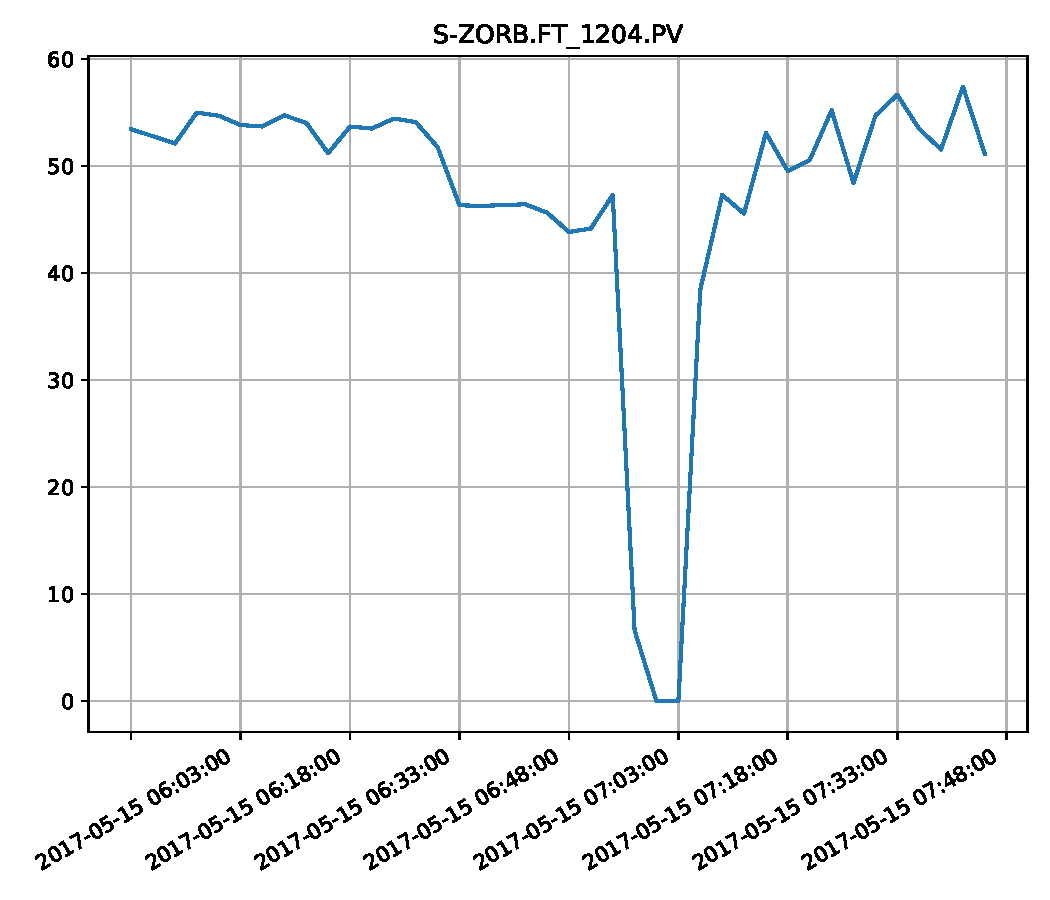
\includegraphics[height=0.3\textheight]{313-fill-1}
        \subcaption{S-ZORB.FT\_1204.PV}
    \end{minipage}
    \begin{minipage}[c]{0.48\textwidth}
        \centering
        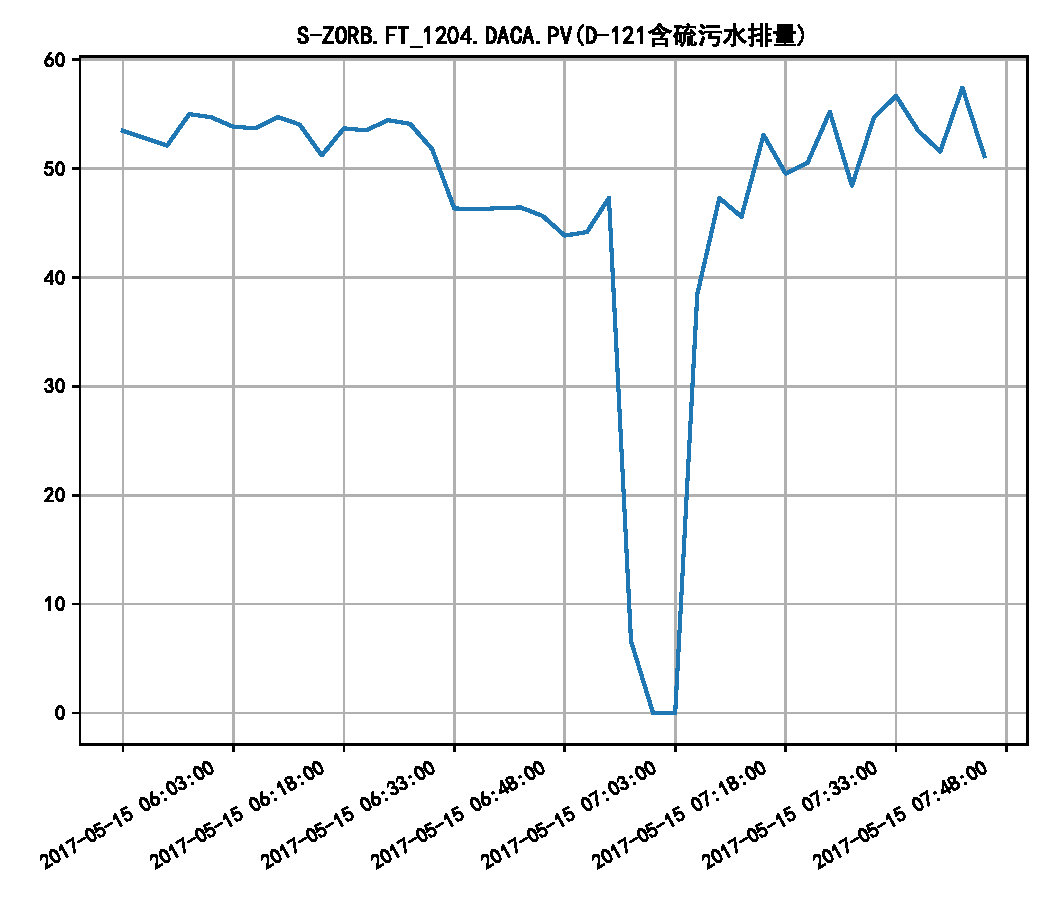
\includegraphics[height=0.3\textheight]{313-fill-2}
        \subcaption{D-121含硫污水排量}
    \end{minipage}
    \caption{?????????}
\end{figure}



% \begin{figure}[!htb]
% 	\centering
% 	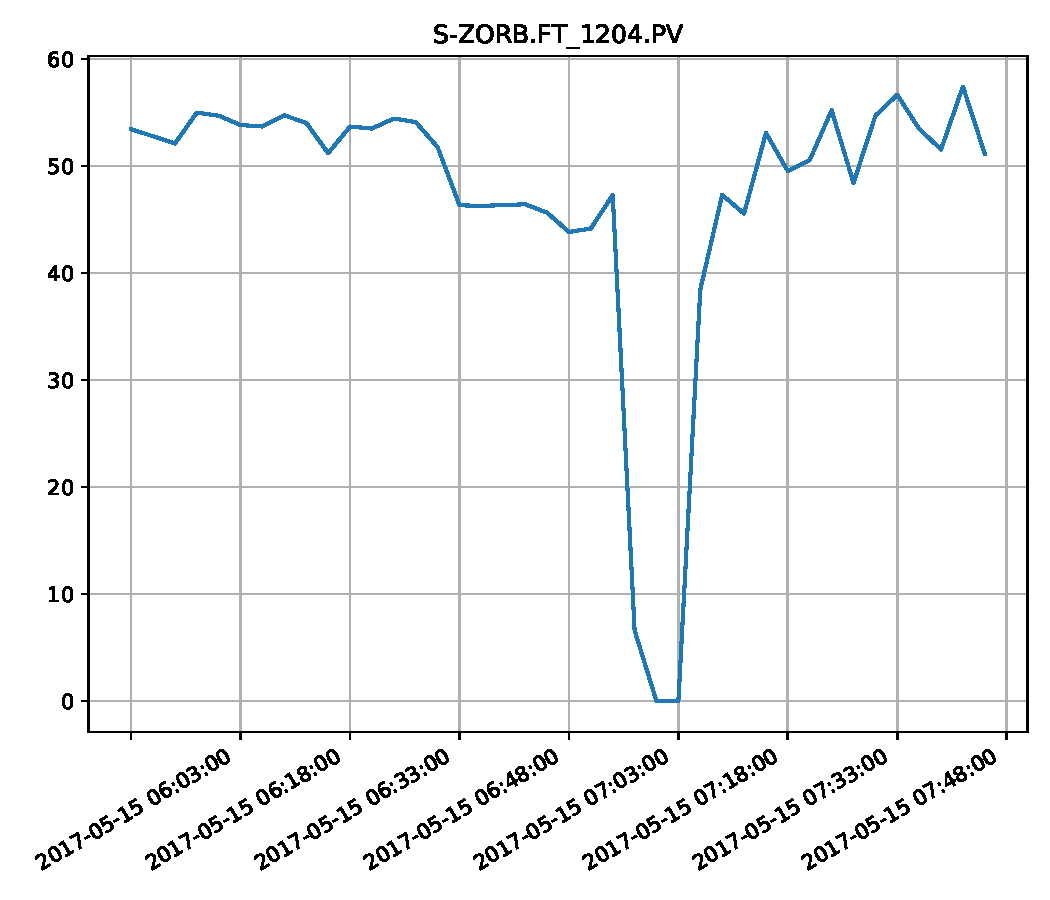
\includegraphics[width=.7\textwidth]{313-fill-1}
% 	\caption{S-ZORB.FT\_1204.PV}
% \end{figure}


% \begin{figure}[!htb]
% 	\centering
% 	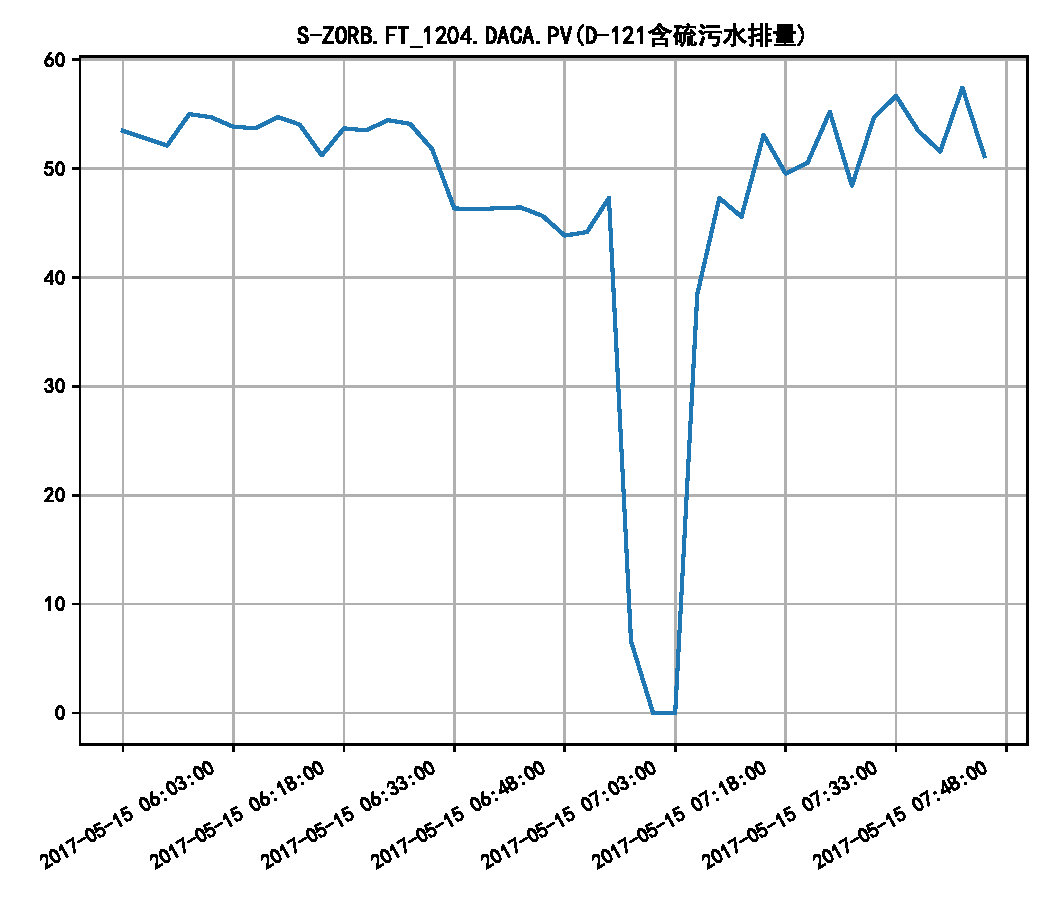
\includegraphics[width=.7\textwidth]{313-fill-2}
% 	\caption{D-121含硫污水排量}
% \end{figure}



处理2:对时序上杂乱或呈周期趋势的含空值变量做删除操作


\begin{figure}[htb]
    \centering
    \begin{minipage}[c]{0.48\textwidth}
        \centering
        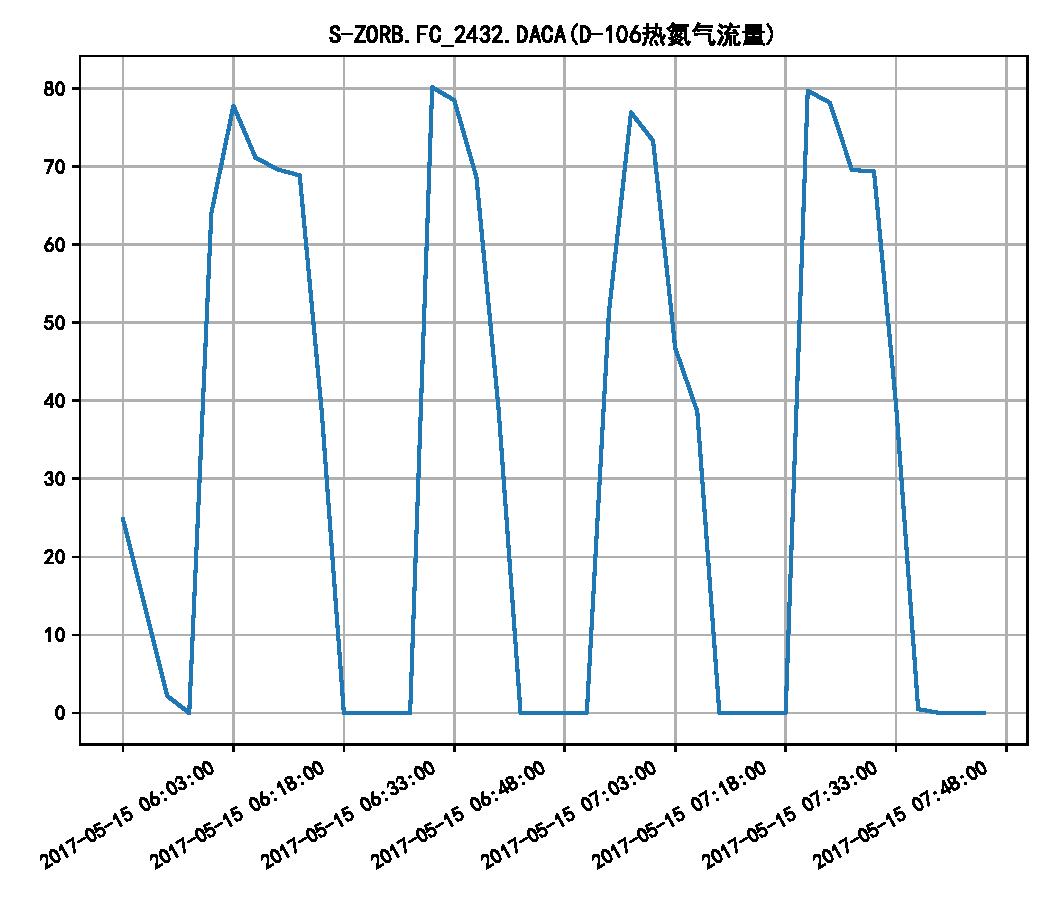
\includegraphics[height=0.3\textheight]{313-del-1}
        \subcaption{D-106热氮气流量}
    \end{minipage}
    \begin{minipage}[c]{0.48\textwidth}
        \centering
        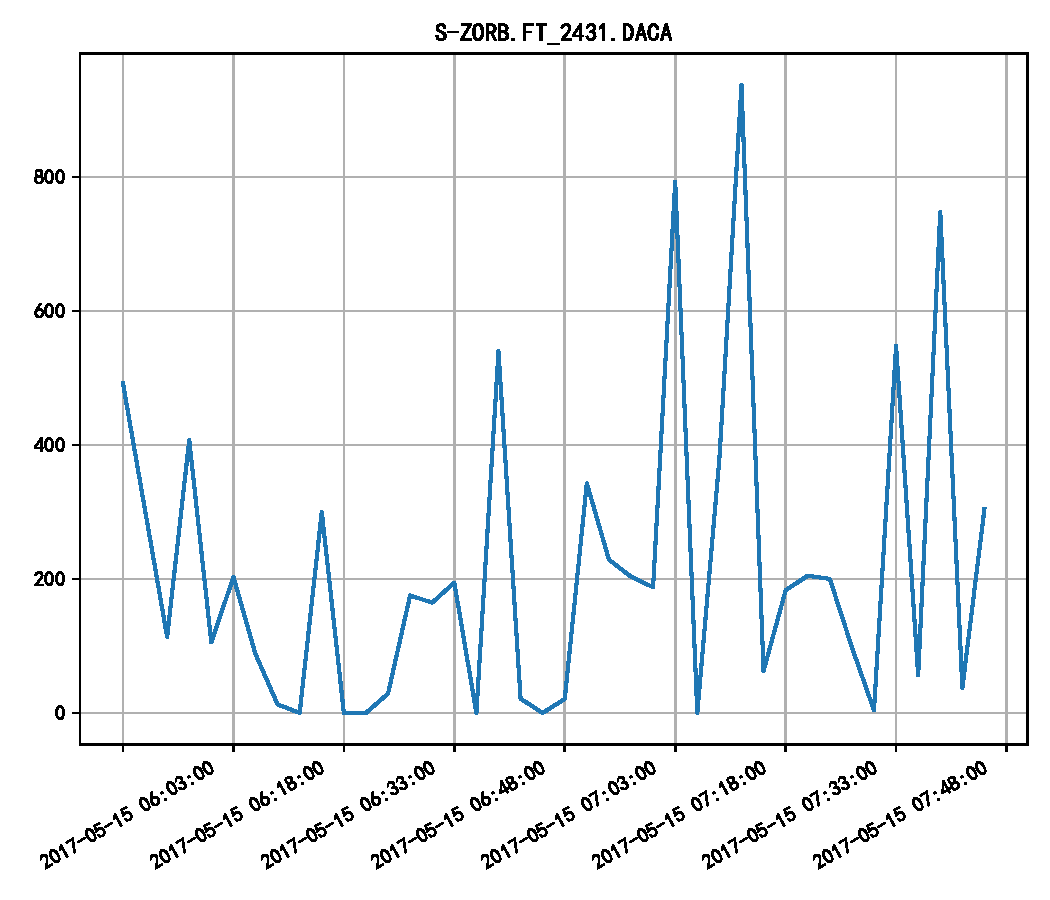
\includegraphics[height=0.3\textheight]{313-del-2}
        \subcaption{S-ZORB.FT\_2431.DACA}
    \end{minipage}
     \begin{minipage}[c]{0.48\textwidth}
        \centering
        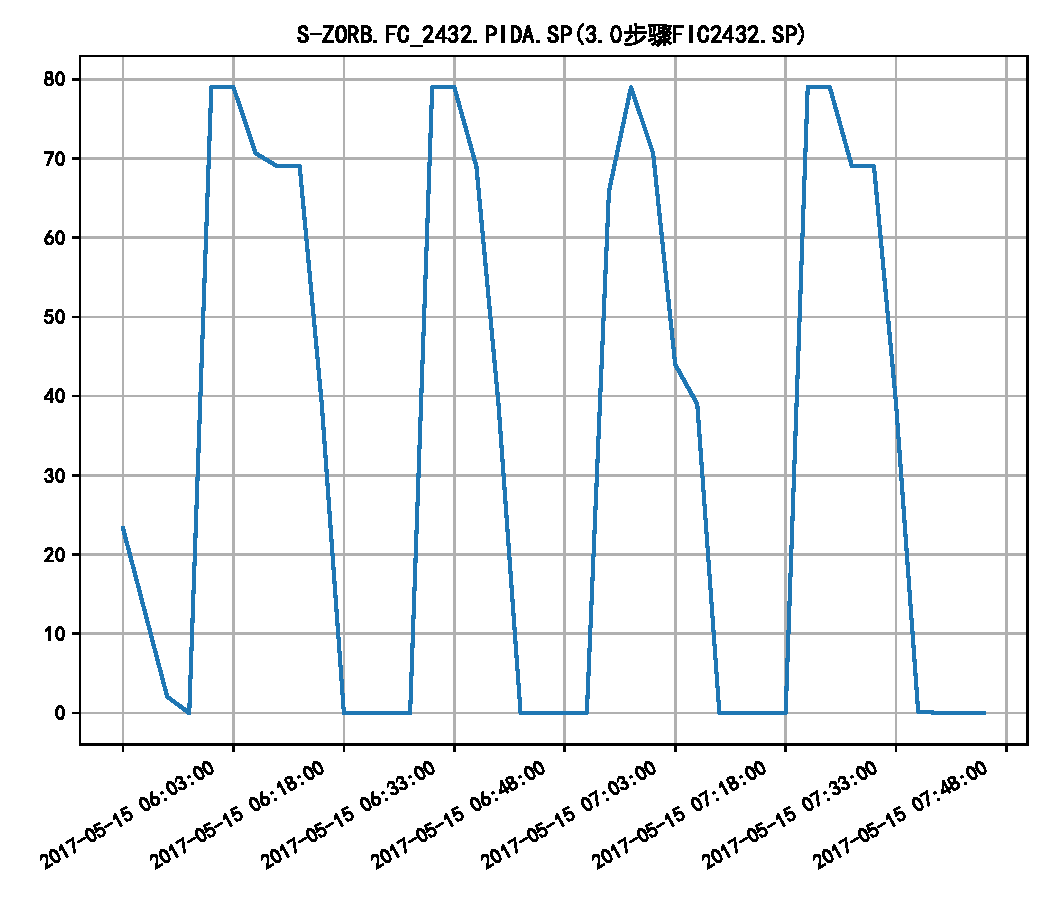
\includegraphics[height=0.3\textheight]{313-del-3}
        \subcaption{3.0步骤FIC2432.SP}
    \end{minipage}
    \caption{?????????}
\end{figure}


% \begin{figure}[!htb]
% 	\centering
% 	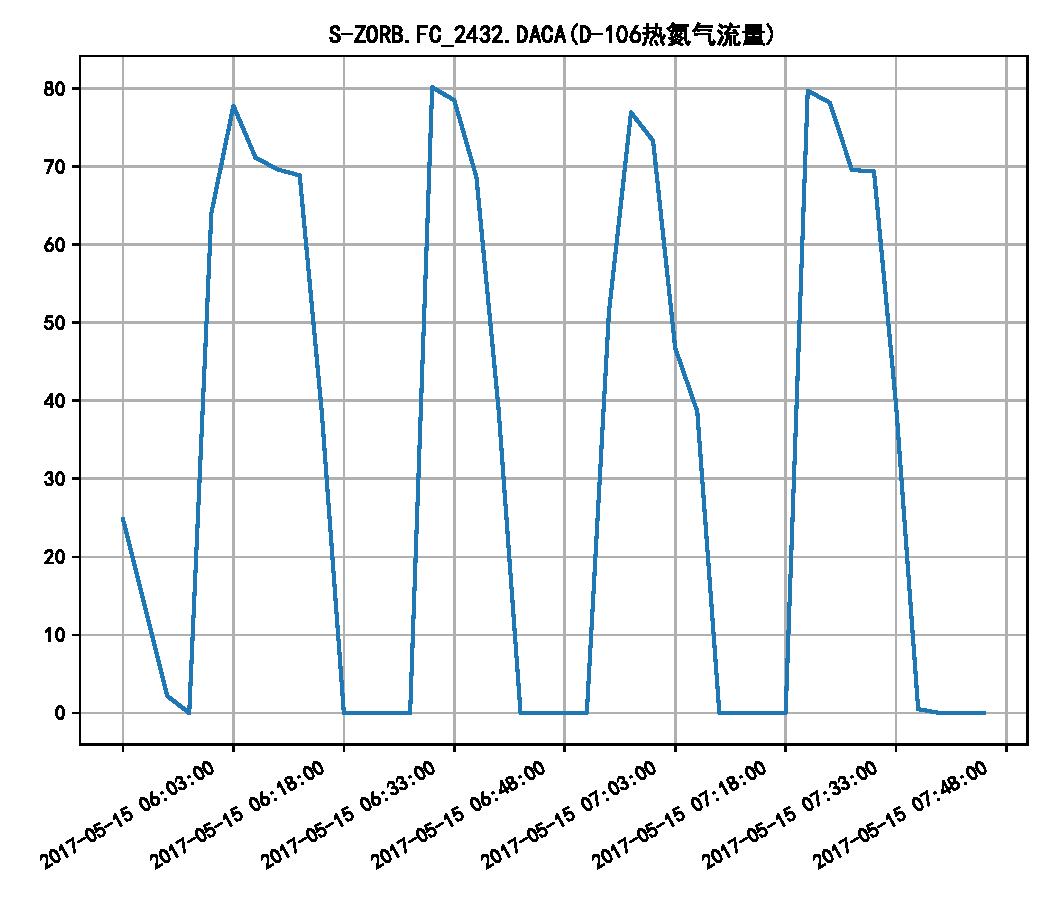
\includegraphics[width=.7\textwidth]{313-del-1}
% 	\caption{D-106热氮气流量}
% \end{figure}


% \begin{figure}[!htb]
% 	\centering
% 	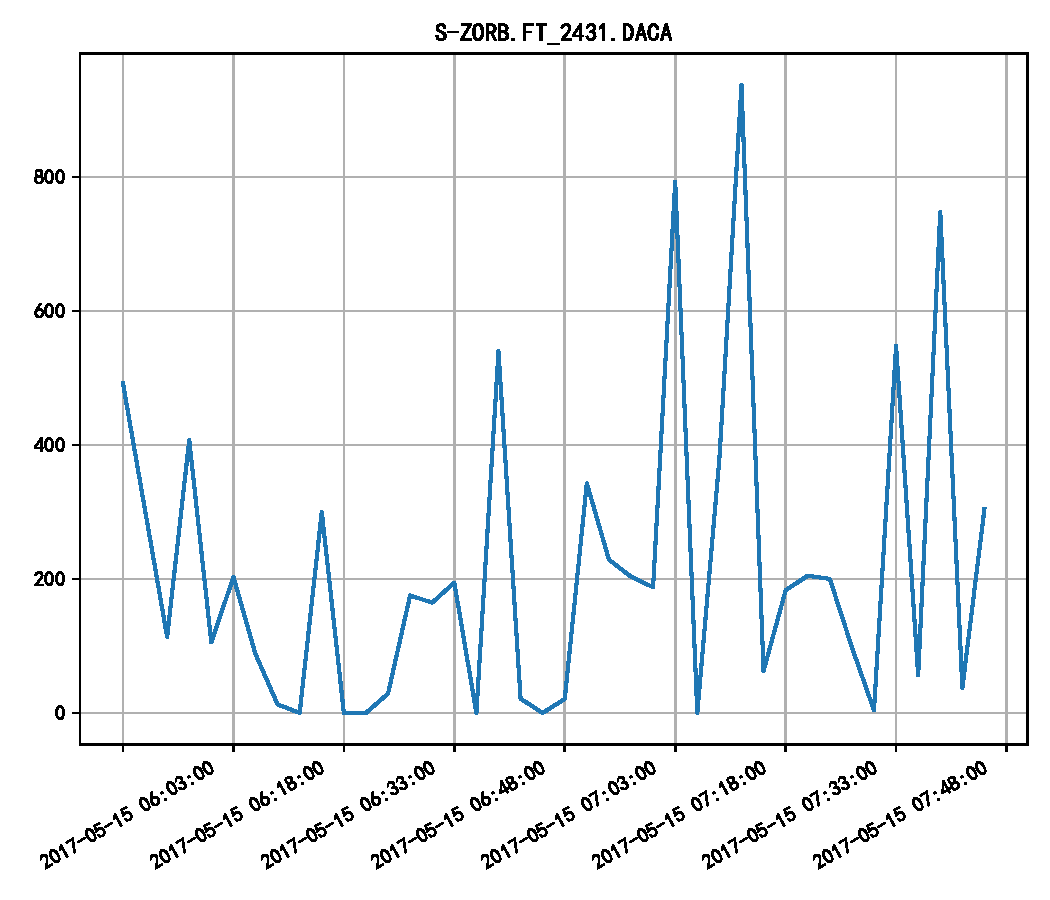
\includegraphics[width=.7\textwidth]{313-del-2}
% 	\caption{S-ZORB.FT\_2431.DACA}
% \end{figure}


% \begin{figure}[!htb]
% 	\centering
% 	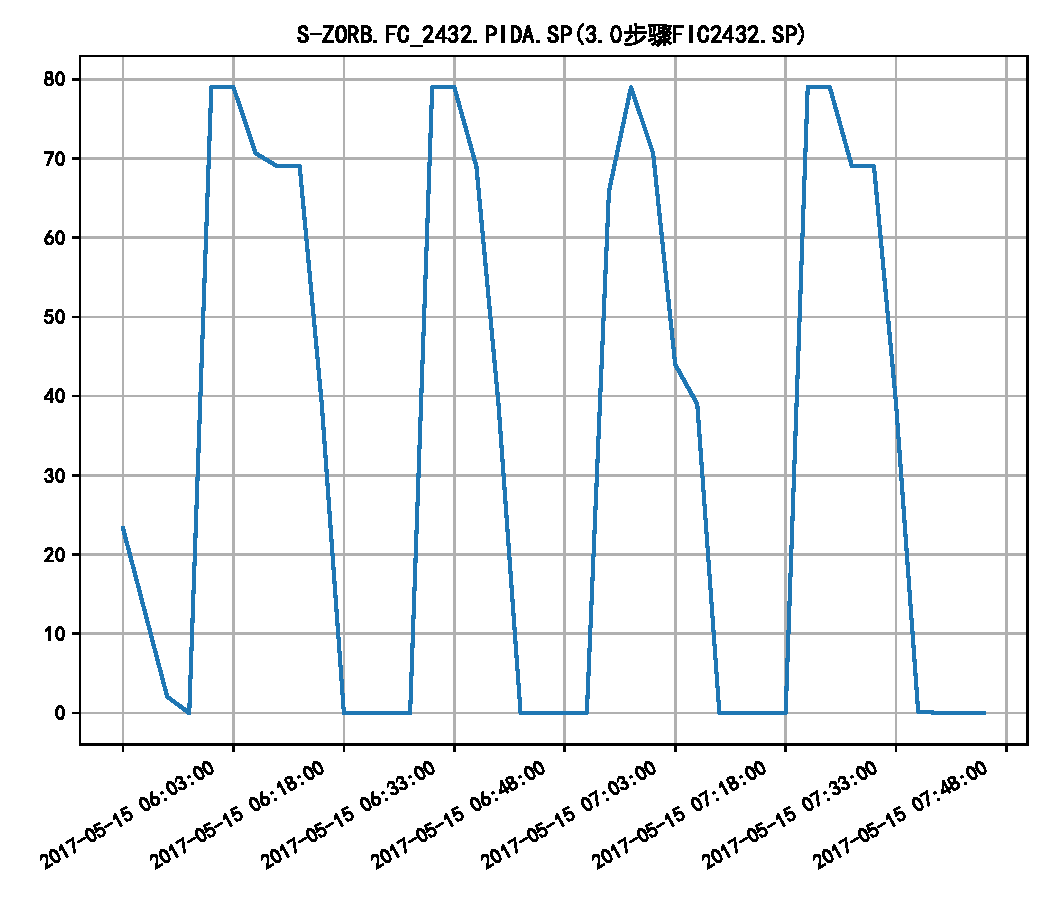
\includegraphics[width=.7\textwidth]{313-del-3}
% 	\caption{3.0步骤FIC2432.SP}
% \end{figure}


\FloatBarrier
\subsubsection{剔除不在操作范围内的样本}

考虑到“325个样本数据.xlsx”中的很多样本已经超出了“354个操作变量信息.xlsx”所规定的范围,我们进行了简单的处理,用“325个样本数据”中每个操作变量的最大与最小值来扩充“354个操作变量信息”中操作变量的范围,并用扩充后的操作变量范围代替原操作变量范围。

经过计算,285样本数据中所有的采样数据都在操作变量范围内,而313样本数据仅有1个采样数据的所有变量在操作变量范围内。经过综合考虑,我们决定用以下公式来计算一个采样样本操出操作变量范围的程度:

\begin{equation}
	InvalidDegree=\sum^M_j{\frac{Exceed_j}{Upper_j - Lower_j}}
	\label{eq:range-invalid-degree}
\end{equation}

其中,$j$表示某采样样本的第$j$个操作变量,$M$表示共有$M$个操作变量, $Upper_j$表示操作变量$j$的上界,$Lower_j$表示操作变量$j$的下界,$Exceed_j$表示操作变量$j$超出范围的大小。

使用上述公式,对313样本的采样数据进行计算,结果如下:

\begin{table}[htb]
	\caption{313样本超出范围程度}\label{tab:001} \centering
	\begin{tabular}{ccc}
	\toprule[1.5pt]
	time &  invalid-degree &  rank \\
	\midrule[1pt]
	2017-05-15 06:57:00 &        1.986283 &     0 \\
	2017-05-15 07:24:00 &        1.868216 &     1 \\
	2017-05-15 07:18:00 &        1.533825 &     2 \\
	2017-05-15 06:33:00 &        1.514671 &     3 \\
	2017-05-15 06:54:00 &        1.298304 &     4 \\
	2017-05-15 06:51:00 &        1.057390 &     5 \\
	2017-05-15 07:21:00 &        0.876193 &     6 \\
	2017-05-15 07:51:00 &        0.866200 &     7 \\
	2017-05-15 07:48:00 &        0.770276 &     8 \\
	2017-05-15 07:54:00 &        0.658065 &     9 \\
	\bottomrule[1.5pt]
\end{tabular}
\end{table}


经过??????????????,我们决定以$InvalidDegree >= 1$为阈值,删除满足其条件的所有采样样本。



\FloatBarrier
\subsubsection{用3$\sigma$准则删除异常样本}

3$\sigma$准则:设对被测量变量进行等精度测量,得到$x_1, x_2, \ldots, x_n$,算出其算术平均值$x$及剩余误差$v_i=x_i-x (i=1, 2, \ldots , n)$,并按贝塞尔公式算出标准误差$\sigma$,若某个测量值$x_b$的剩余误差$v_b ( 1 <= b <= n )$,满足 $|v_b| = | x_b - x | > 3\sigma$,则认为$x_b$是含有粗大误差值的坏值,应予剔除。贝塞尔公式如下:

\begin{equation}\label{eq:3sigma}
	\sigma = [\frac{1}{n-1}\sum_{i=1}^{n}v_i^2]^{\frac{1}{2}} = \{\frac{[\sum^n_{i=1}x_i^2 - (\sum^n_{i=1}x_i)^2/n]}{n-1}\}^{\frac{1}{2}}
\end{equation}

根据上述公式,285样本的所有采样都满足3$\sigma$准则,而313样本有27个采样不满足其条件,故删除这些不满足条件的变量。


\FloatBarrier
\subsubsection{对工业数据中的空值变量进行处理}

通过前述操作,将313样本和285样本经过处理后加入到325个样本的工业数据中,并将4.1.2处理2(引用)中删除的变量设置为 $NaN$ ,待进一步的处理。

考虑到工业设备????????????,我们认为0代表了工业数据中的空值。对于不同类型的情况,我们制定了3种处理空值的策略:

\begin{equation}\label{eq:empty-strategies}
\left\{
\begin{aligned}
delete \ column, \ & if \ len(EmptyElements)>50 \ and \ mean(vector)>5 \\  
delete \ element, \ & if \ len(EmptyElements)<50 \ and \ mean(vector)>5\\  
do \ not \ process, \ & if \ mean(vector)<=5
\end{aligned}
\right.
\end{equation}

根据公式(引用)中,如果某列空值元素的长度 $len(EmptyElements)$ 大于50,并且这列元素的均值 $ mean(vector)$ 大于5,说明空值较多,做空值填充的意义不大,应该将此列删除。如果某列空值元素的长度小于50,并且这列元素的均值大于5,说明空值相对较少,可以通过做空值填充保留下来。如果这列元素的均值小于等于5,说明这列元素基本为0,0可能不是这列元素的空值,所以不做处理。
三种策略的处理结果数据如下:

\begin{figure}[htb]
	\centering
	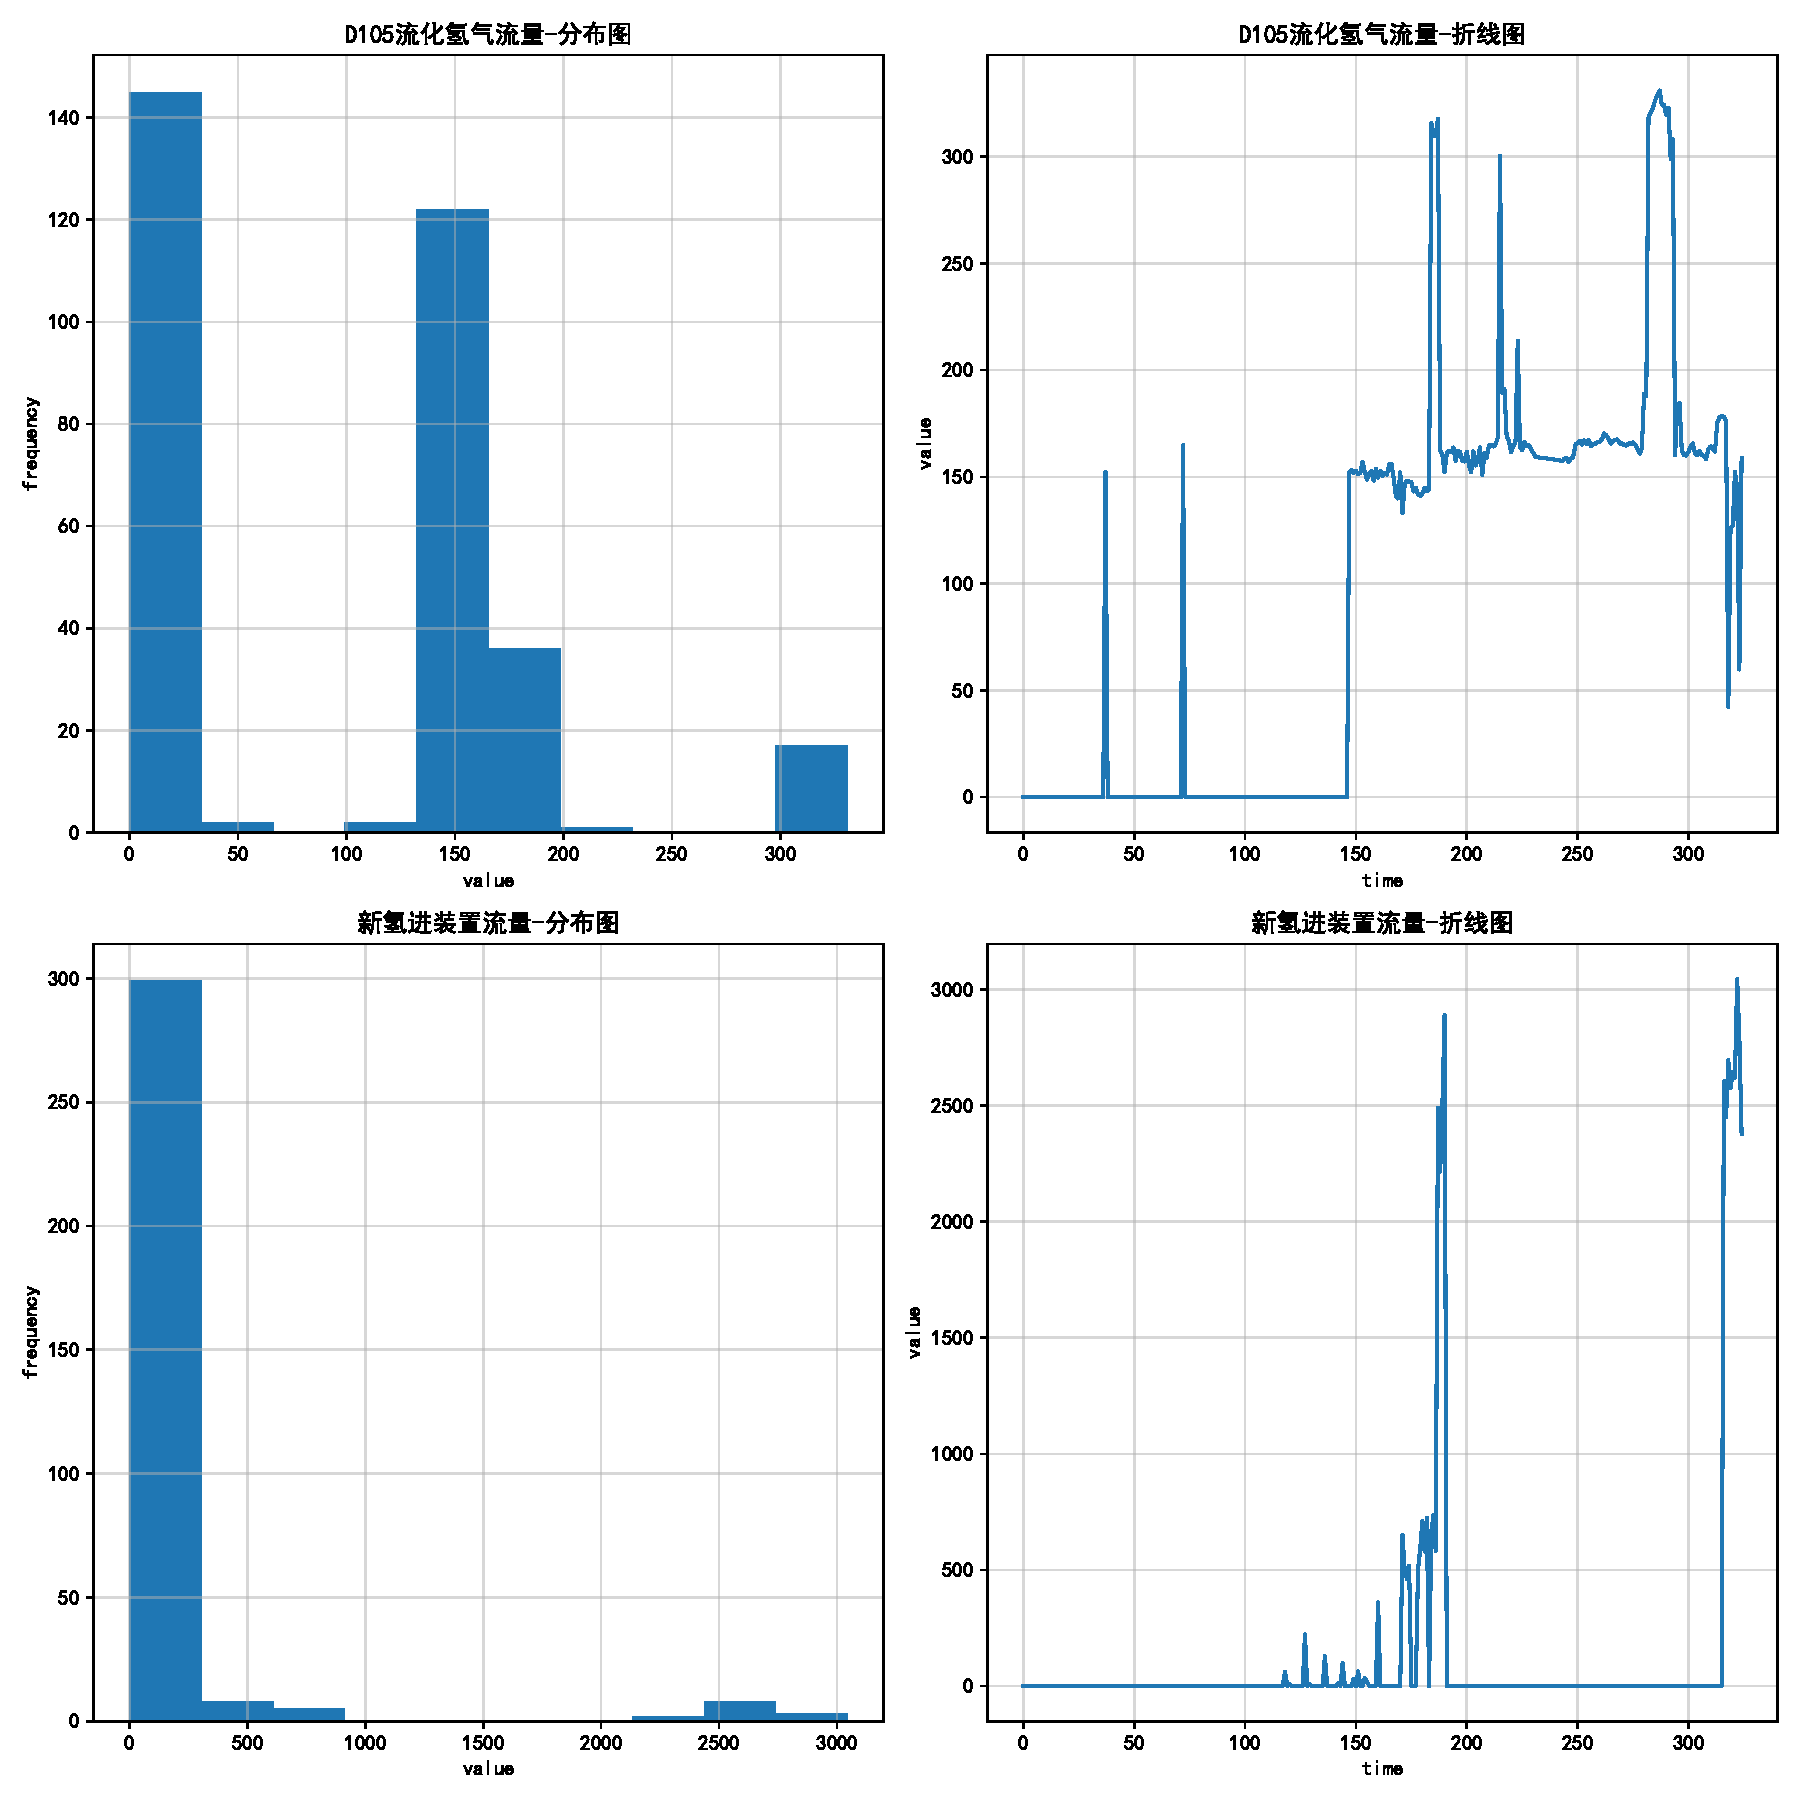
\includegraphics[width=1.0\textwidth]{strategy-1}
	\caption{策略1}
\end{figure}


\begin{figure}[htb]
	\centering
	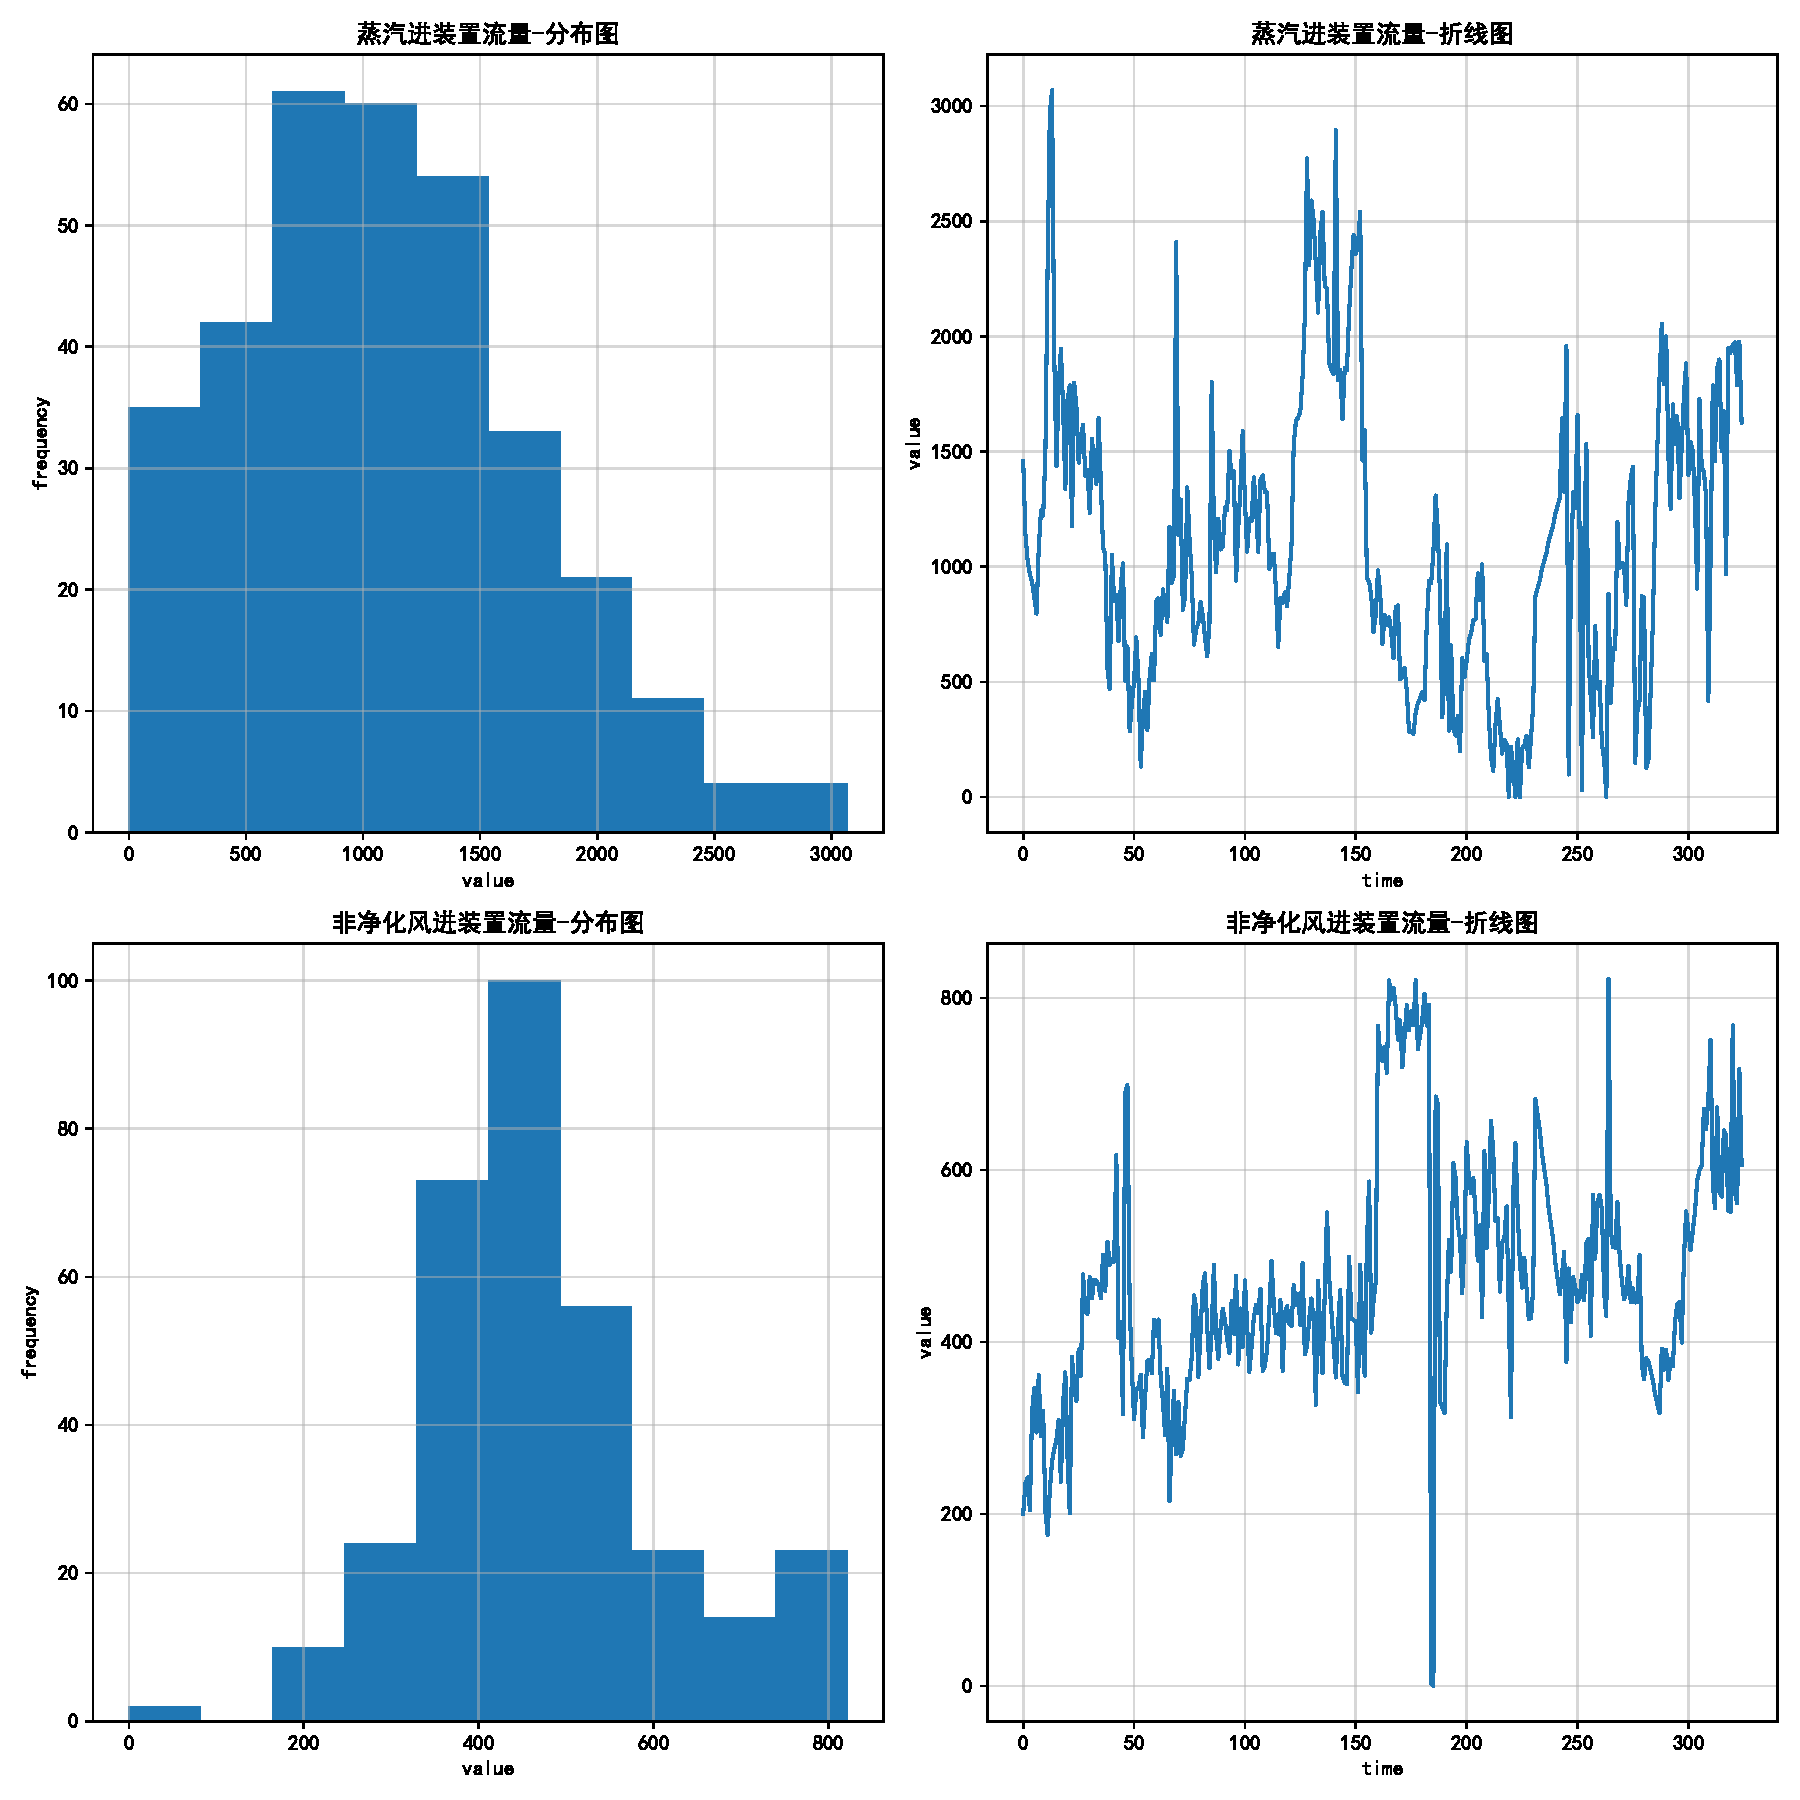
\includegraphics[width=1.0\textwidth]{strategy-2}
	\caption{策略2}
\end{figure}


\begin{figure}[htb]
	\centering
	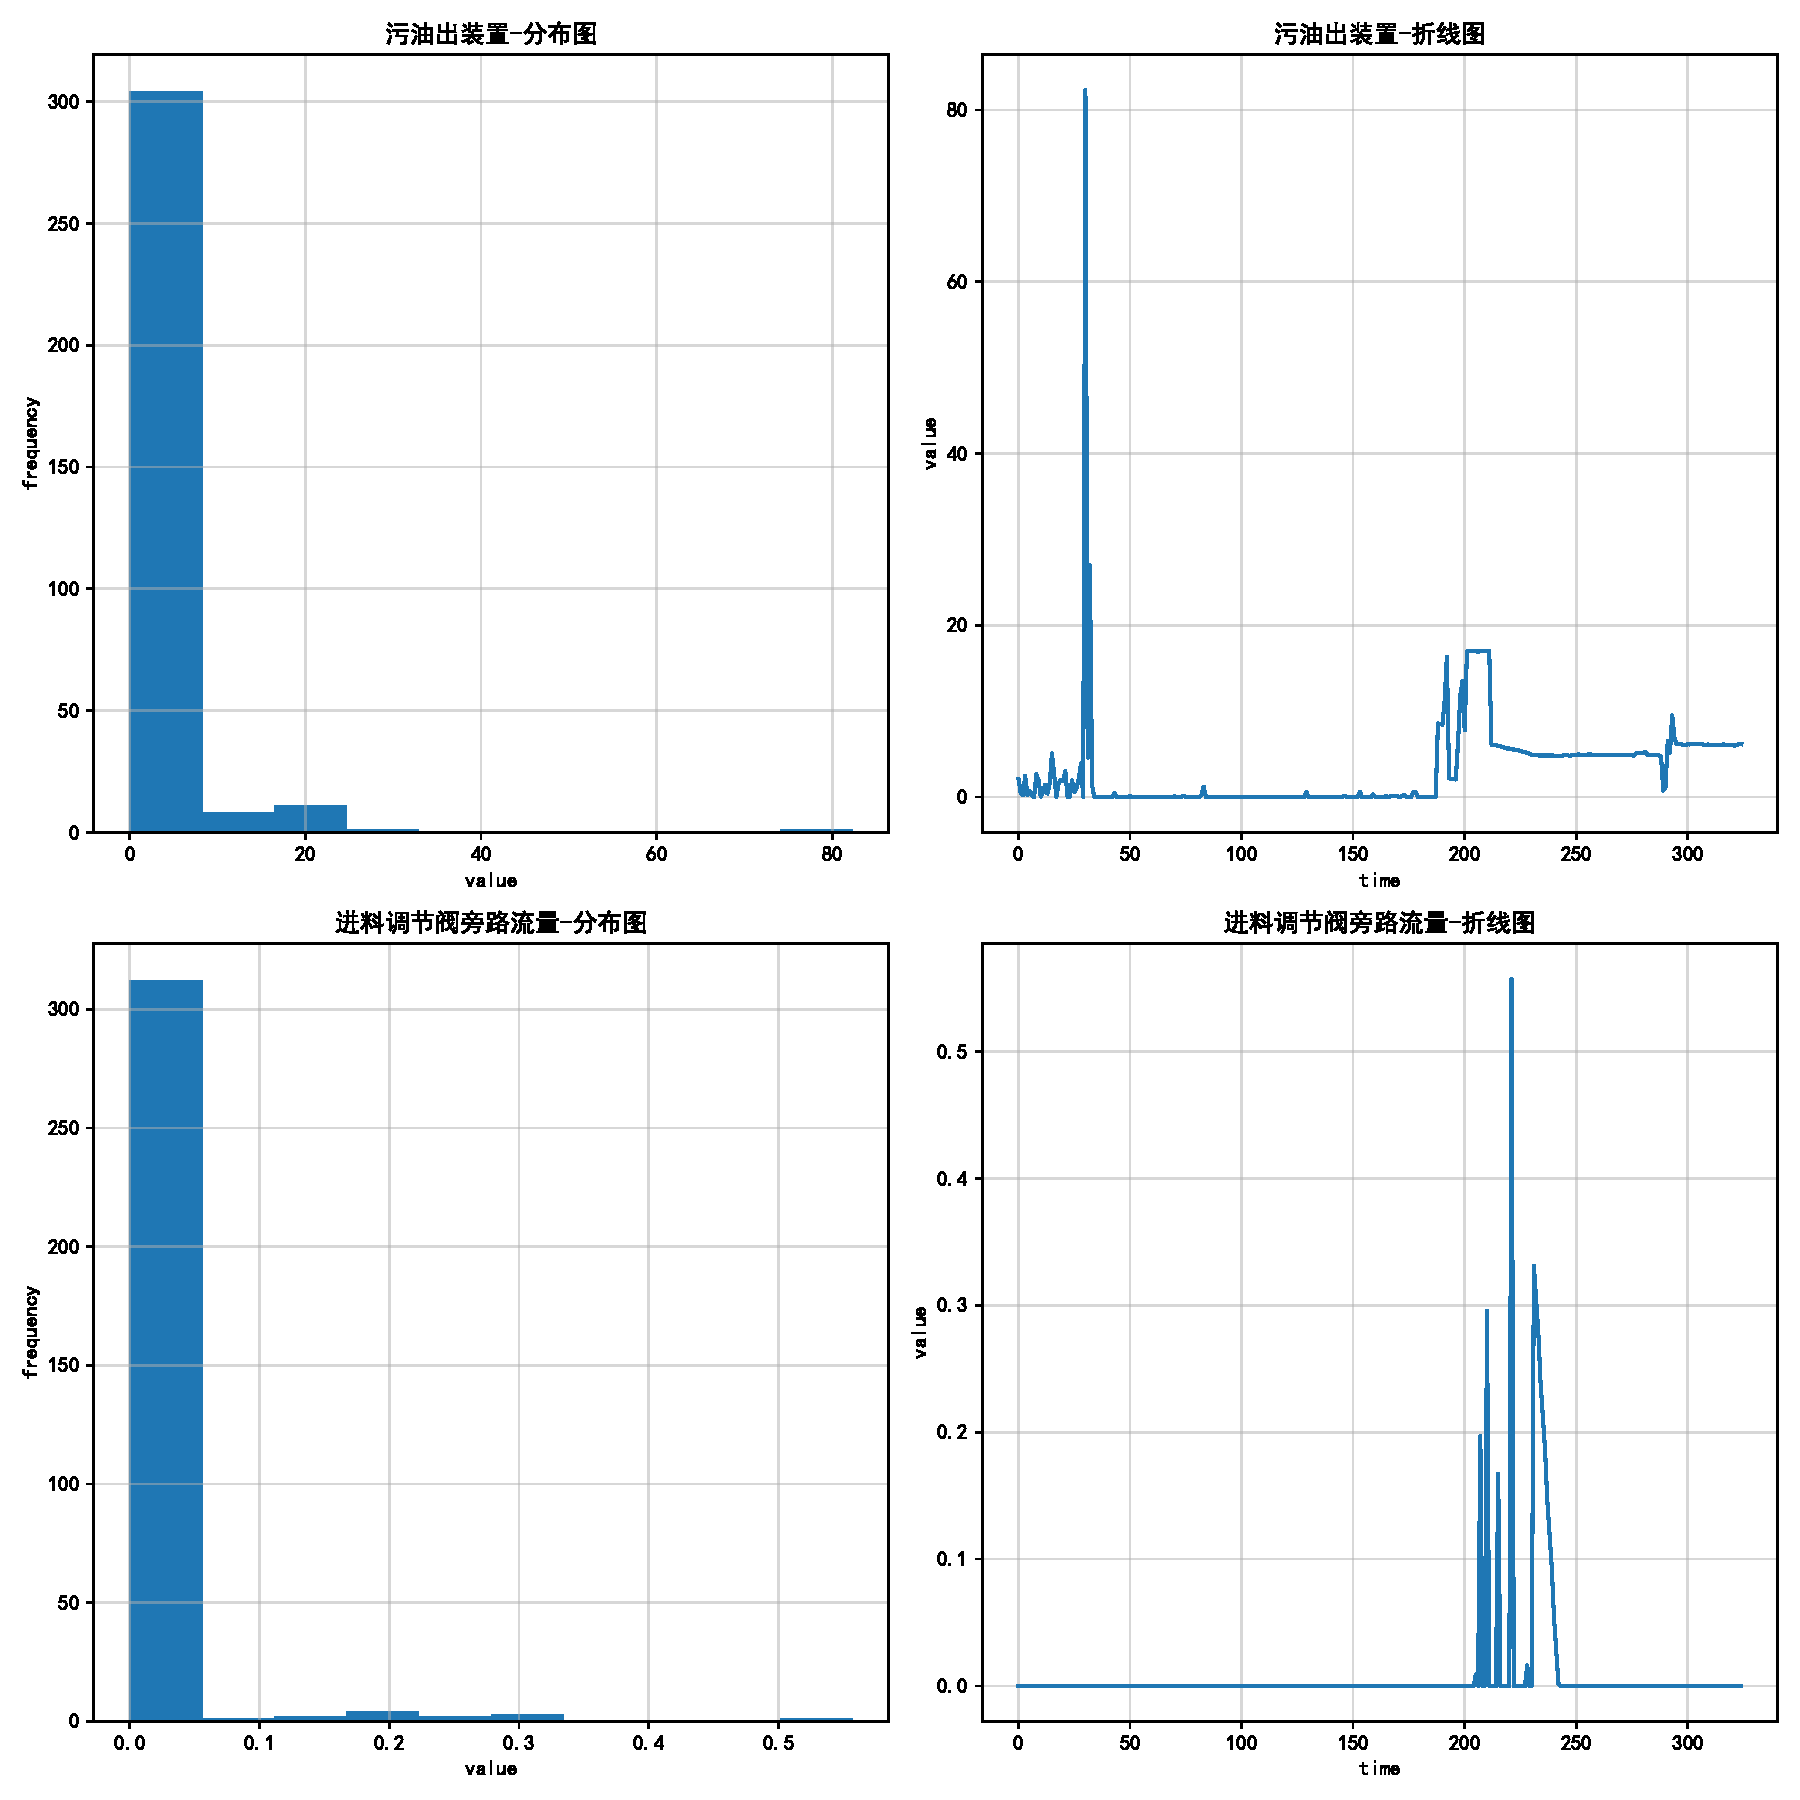
\includegraphics[width=1.0\textwidth]{strategy-3}
	\caption{策略3}
\end{figure}

\FloatBarrier
\subsection{问题二:寻找建模主要变量}
\FloatBarrier
\subsubsection{问题分析}


????????????????????????????
由于催化裂化汽油精制过程是连续的,虽然操作变量每3 分钟就采样一次,但辛烷值(因变量)的测量比较麻烦,一周仅2次无法对应。但根据实际情况可以认为辛烷值的测量值是测量时刻前两小时内操作变量的综合效果,因此预处理中取操作变量两小时内的平均值与辛烷值的测量值对应。这样产生了325个样本(见附件一)。

建立降低辛烷值损失模型涉及包括7个原料性质、2个待生吸附剂性质、2个再生吸附剂性质、2个产品性质等变量以及另外354个操作变量(共计367个变量),工程技术应用中经常使用先降维后建模的方法,这有利于忽略次要因素,发现并分析影响模型的主要变量与因素。因此,请你们根据提供的325个样本数据(见附件一),通过降维的方法从367个操作变量中筛选出建模主要变量,使之尽可能具有代表性、独立性(为了工程应用方便,建议降维后的主要变量在30个以下),并请详细说明建模主要变量的筛选过程及其合理性。(提示:请考虑将原料的辛烷值作为建模变量之一)。


\FloatBarrier
\subsubsection{通过特征筛选获取主要变量}

\begin{figure}[htb]
	\centering
	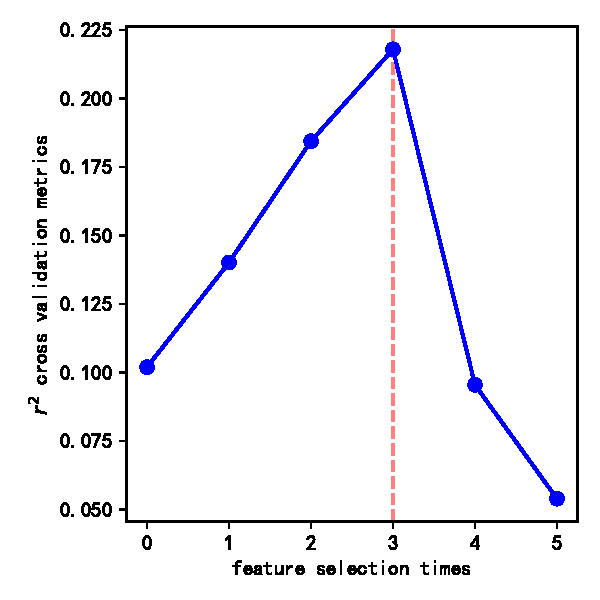
\includegraphics[width=.7\textwidth]{feature-selection-perfs}
	\caption{特征筛选n次后剩余特征数}
\end{figure}

\begin{figure}[htb]
	\centering
	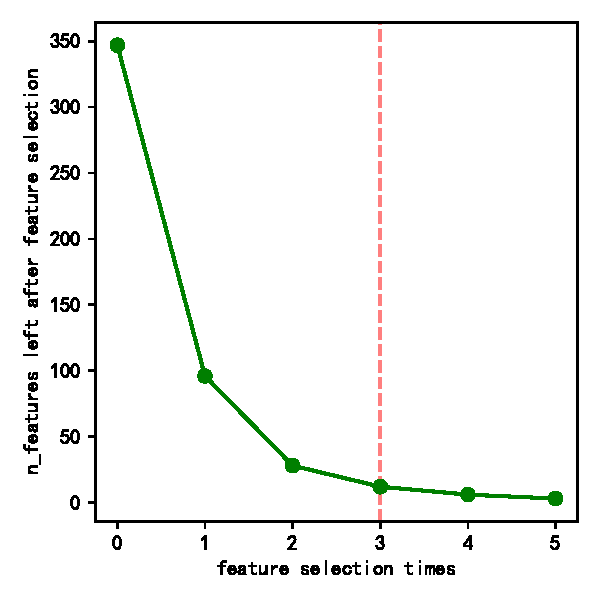
\includegraphics[width=.7\textwidth]{feature-selection-feats}
	\caption{特征筛选次数与$r^2$评价指标的关系}
\end{figure}

\begin{table}[!htbp]
	\caption{特征筛选n次后的各指标}\label{tab:001} \centering
	\begin{tabular}{ccc}
		\toprule[1.5pt]
	feature selection times &  $r^2$ metrics &  n\_features left \\
		\midrule[1pt]
           0 &       0.101955 &              347 \\
			1 &       0.140157 &               96 \\
			2 &       0.184434 &               28 \\
			3 &       0.217998 &               12 \\
			4 &       0.095470 &                6 \\
			5 &       0.053913 &                3 \\
		\bottomrule[1.5pt]
	\end{tabular}
\end{table}


\FloatBarrier
\subsubsection{主要变量数据分析}

\begin{table}[htb]
	\caption{主要变量的特征重要度}\label{tab:001} \centering
	\begin{tabular}{ccccc}
		\toprule[1.5pt]
	 rank & feature importances & percentage (\%) &                  name &        CN name \\
		\midrule[1pt]
    0 &              0.0785 &          12.83 &  S-ZORB.PDT\_1003.DACA &  P-101B入口过滤器差压 \\
	1 &              0.0774 &          12.66 &    S-ZORB.PC\_1001A.PV &    D101原料缓冲罐压力 \\
	2 &              0.0602 &           9.84 &     S-ZORB.TC\_5005.PV &        稳定塔下部温度 \\
	3 &              0.0596 &           9.74 &   S-ZORB.LI\_9102.DACA &        D-204液位 \\
	4 &              0.0515 &           8.42 &   S-ZORB.TE\_1107.DACA &  E-101D壳程出口管温度 \\
	5 &              0.0474 &           7.75 &    S-ZORB.SIS\_TE\_2802 &        D-102温度 \\
	6 &              0.0443 &           7.25 &     S-ZORB.TE\_5202.PV &      精制汽油出装置温度 \\
	7 &              0.0408 &           6.67 &   S-ZORB.TE\_1605.DACA &  F-101出口支管\#4温度 \\
	8 &              0.0390 &           6.37 &   S-ZORB.DT\_2001.DACA &    R-101下部床层压降 \\
	9 &              0.0385 &           6.29 &     S-ZORB.PC\_1603.PV &   加热炉主火嘴瓦斯入口压力 \\
	10 &              0.0379 &           6.20 &     S-ZORB.AT\_5201.PV &     精制汽油出装置硫含量 \\
	11 &              0.0364 &           5.95 &                   RON &            辛烷值 \\
		\bottomrule[1.5pt]
	\end{tabular}
\end{table}

\begin{figure}[htb]
	\centering
	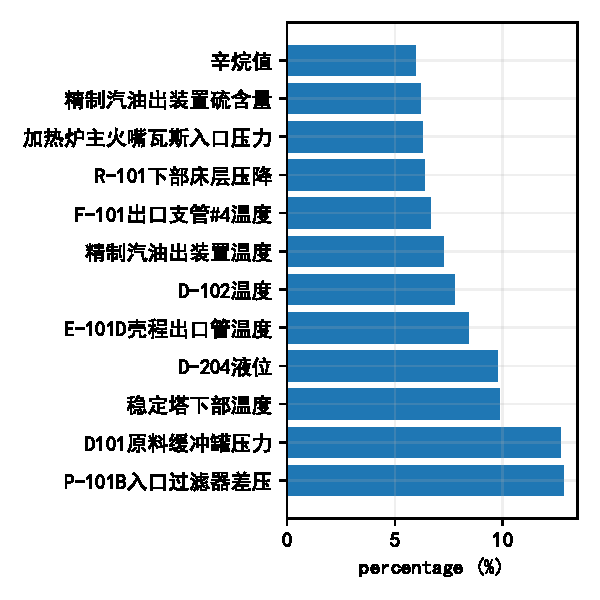
\includegraphics[width=.7\textwidth]{feat-imp}
	\caption{主要变量的特征重要度}
\end{figure}

\begin{figure}[htb]
	\centering
	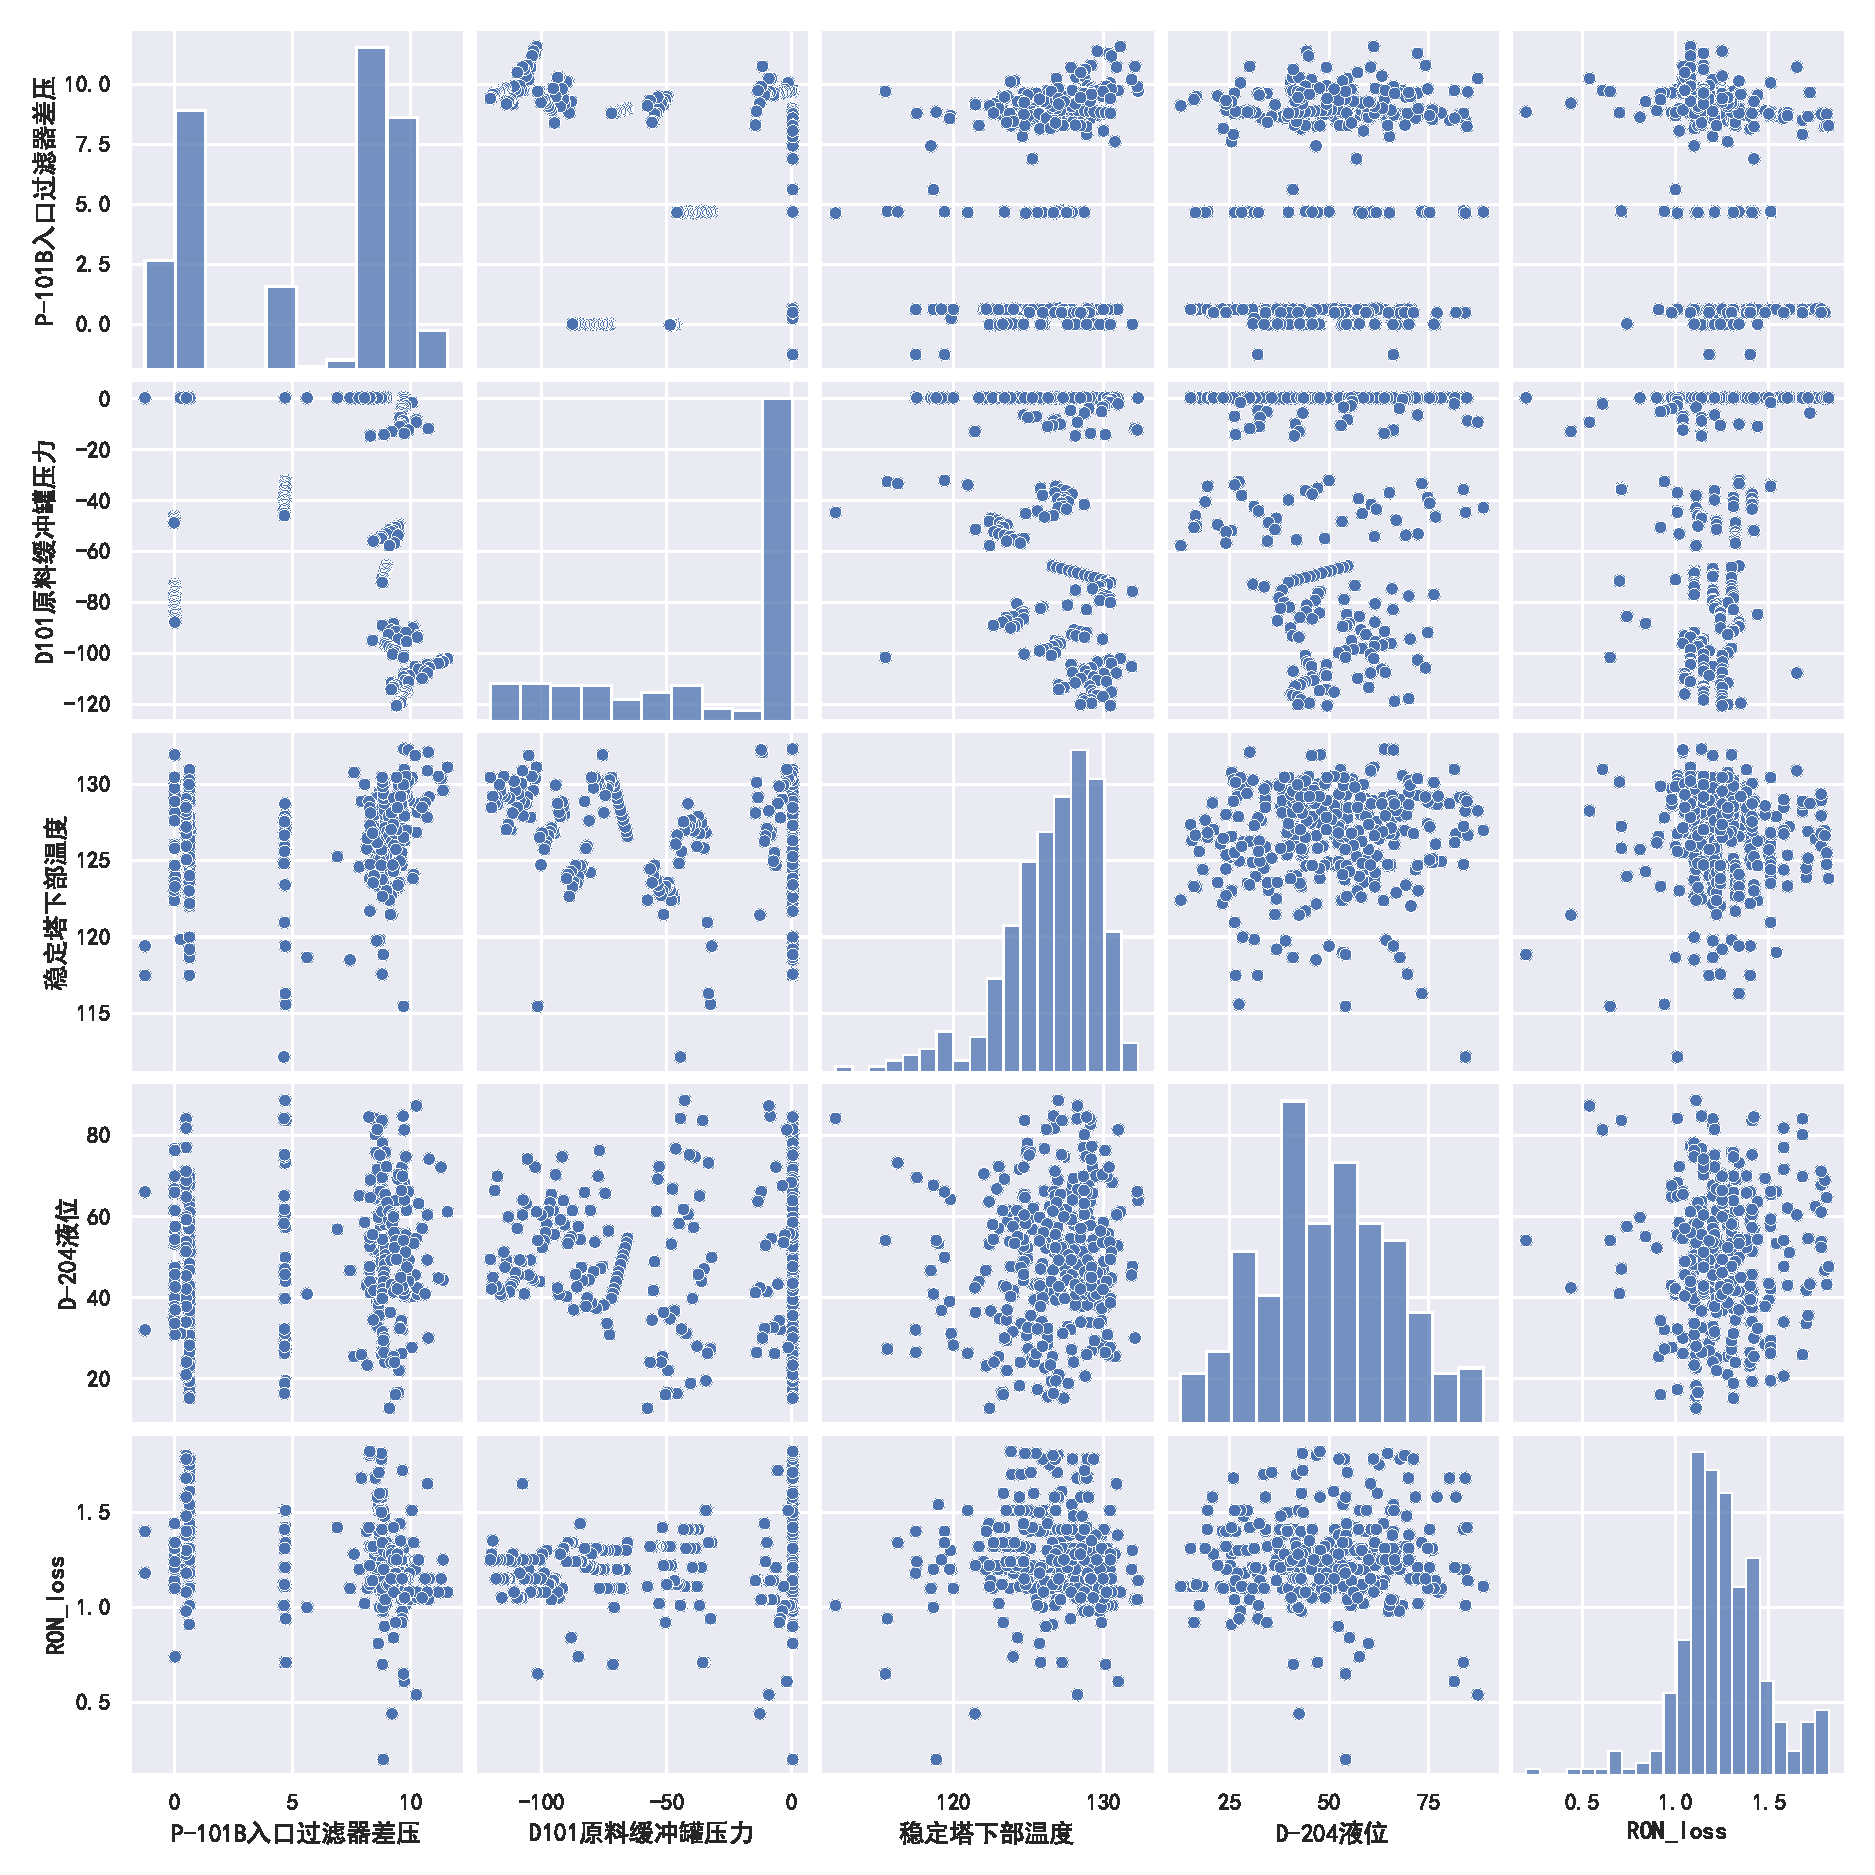
\includegraphics[width=.7\textwidth]{pairplot}
	\caption{相关性矩阵图}
\end{figure}

\begin{figure}[htb]
	\centering
	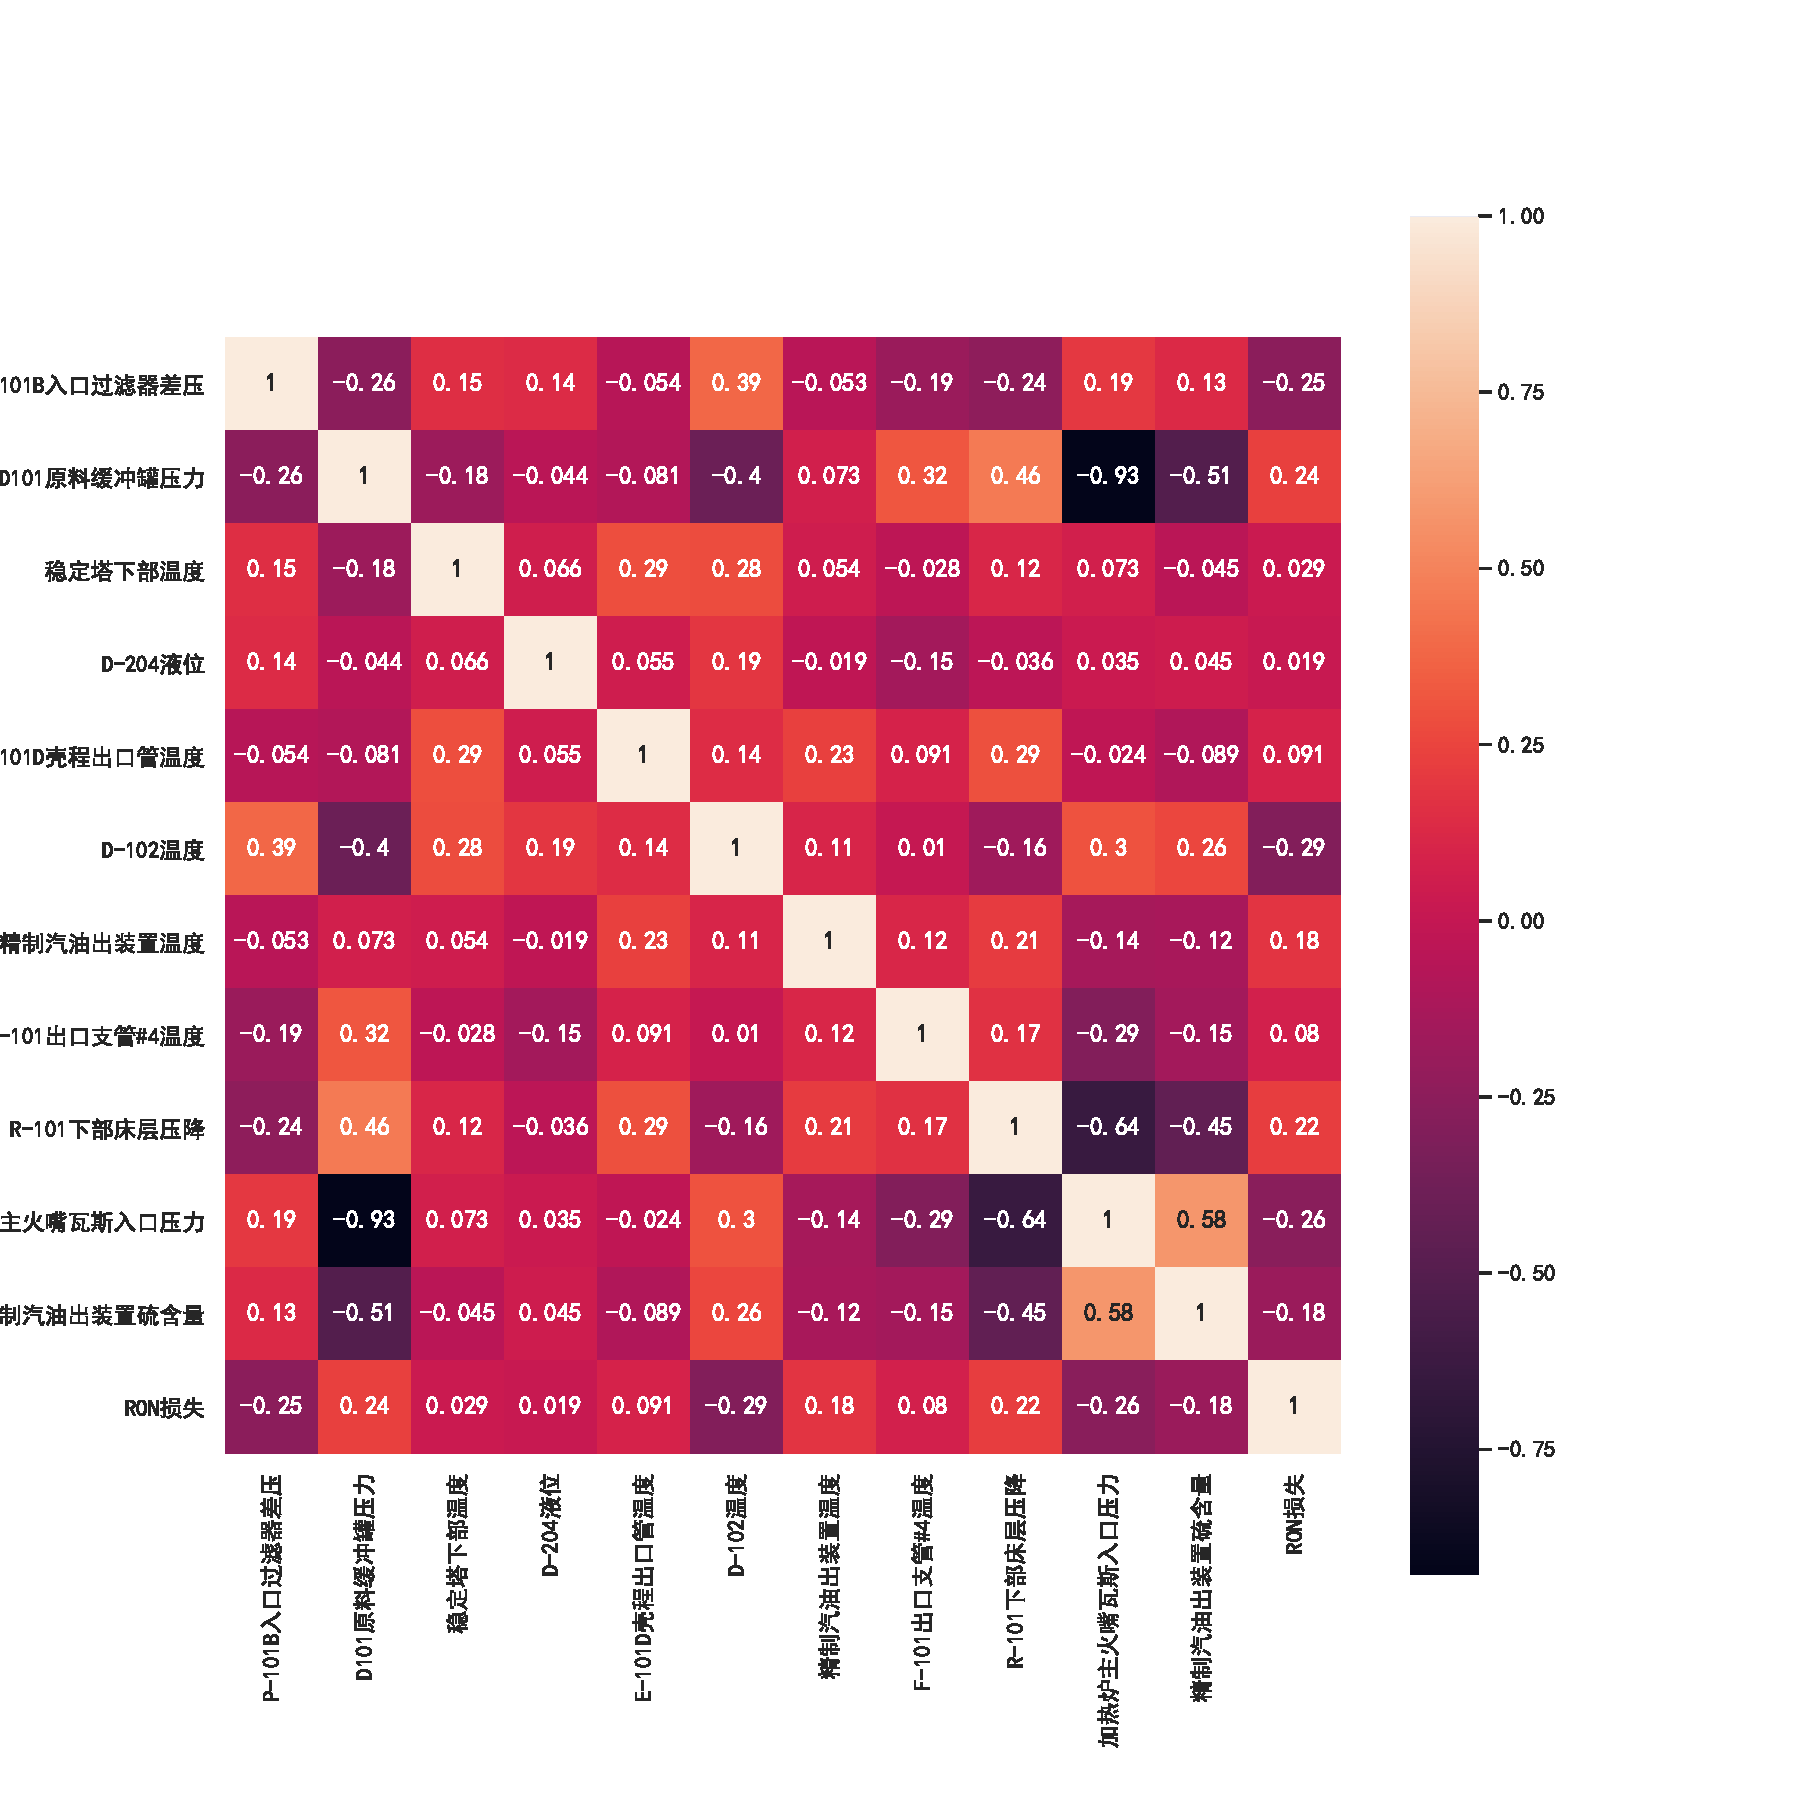
\includegraphics[width=.7\textwidth]{heatmap}
	\caption{热力图}
\end{figure}


\FloatBarrier
\subsection{问题三:建立辛烷值(RON)损失预测模型}

\FloatBarrier
\subsubsection{问题分析}

?????????????????????????????????
采用上述样本和建模主要变量,通过数据挖掘技术建立辛烷值(RON)损失预测模型,并进行模型验证。 


\FloatBarrier
\subsubsection{删除异常样本}

\begin{figure}[htb]
	\centering
	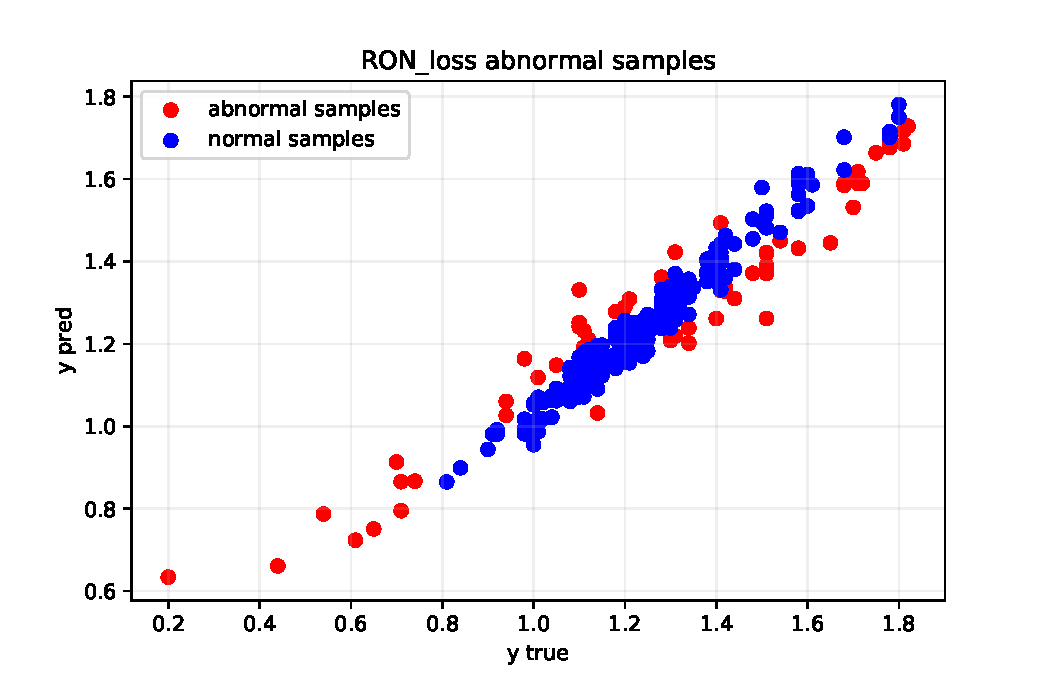
\includegraphics[width=.7\textwidth]{RON-loss-abnormal}
	\caption{删除异常样本}
\end{figure}

\FloatBarrier
\subsubsection{模型训练与验证}

\begin{figure}[htb]
	\centering
	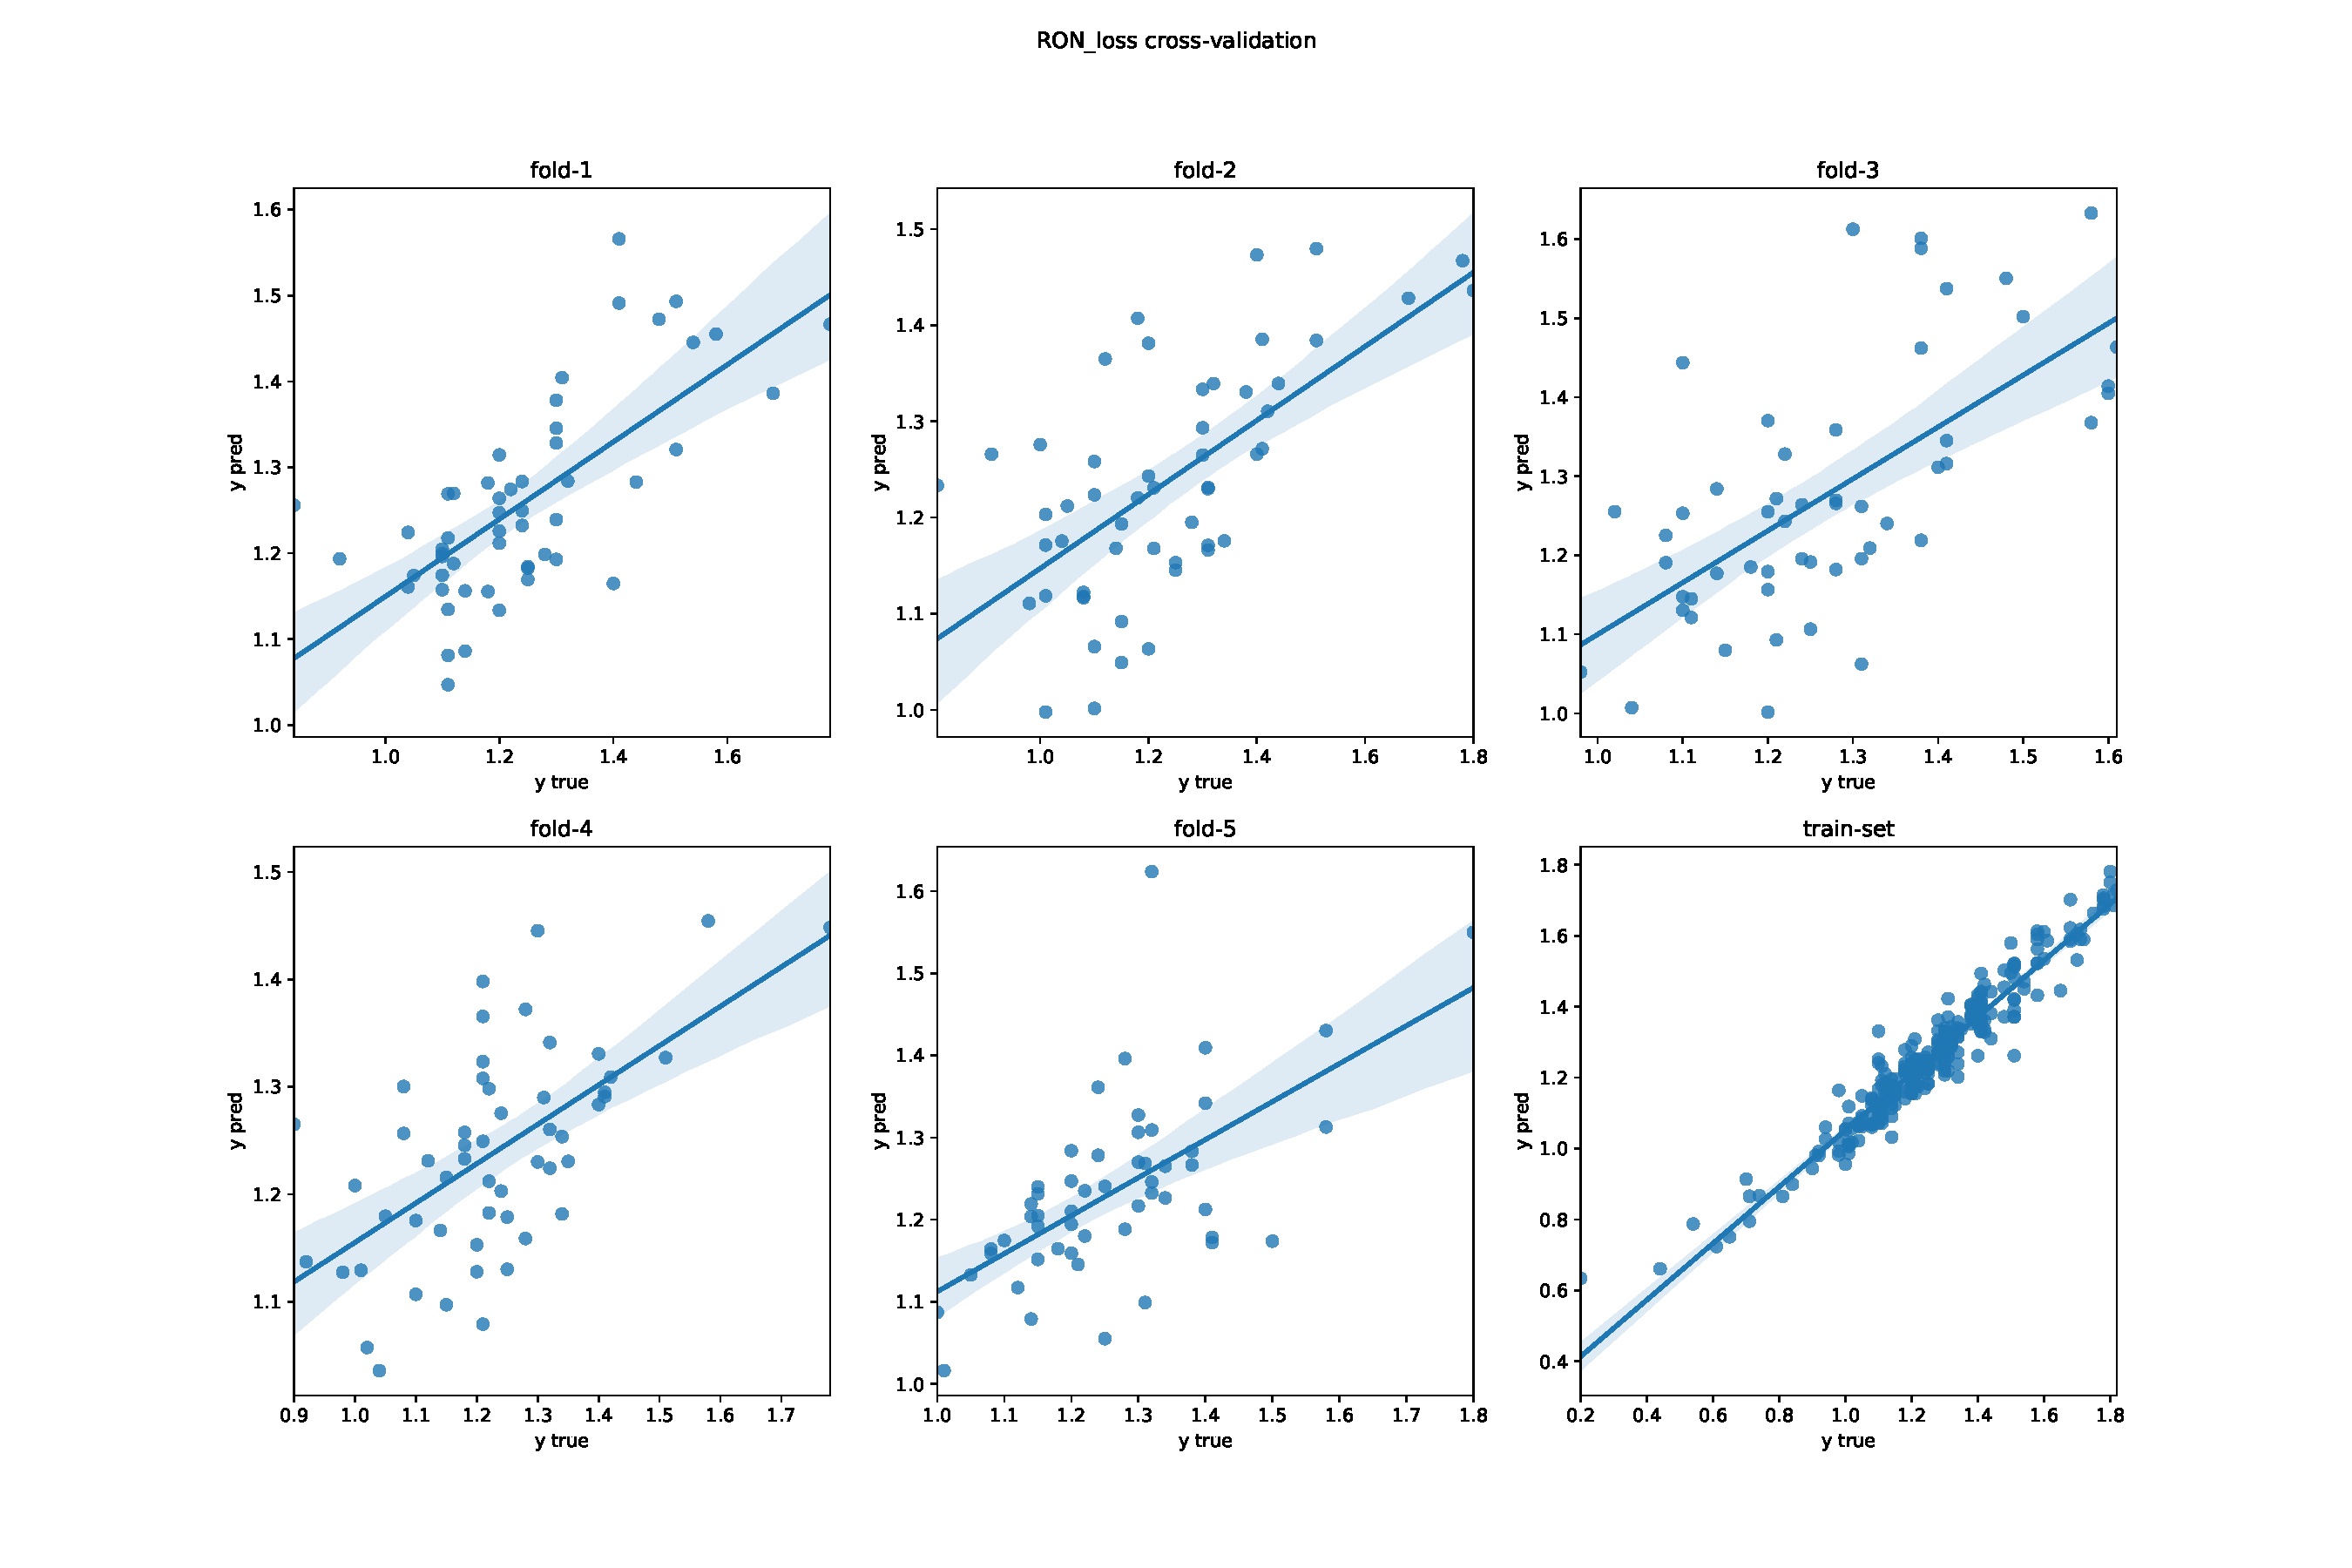
\includegraphics[width=.7\textwidth]{RON-loss-cross-validation}
	\caption{对RON-loss进行交叉验证}
\end{figure}


\begin{figure}[htb]
	\centering
	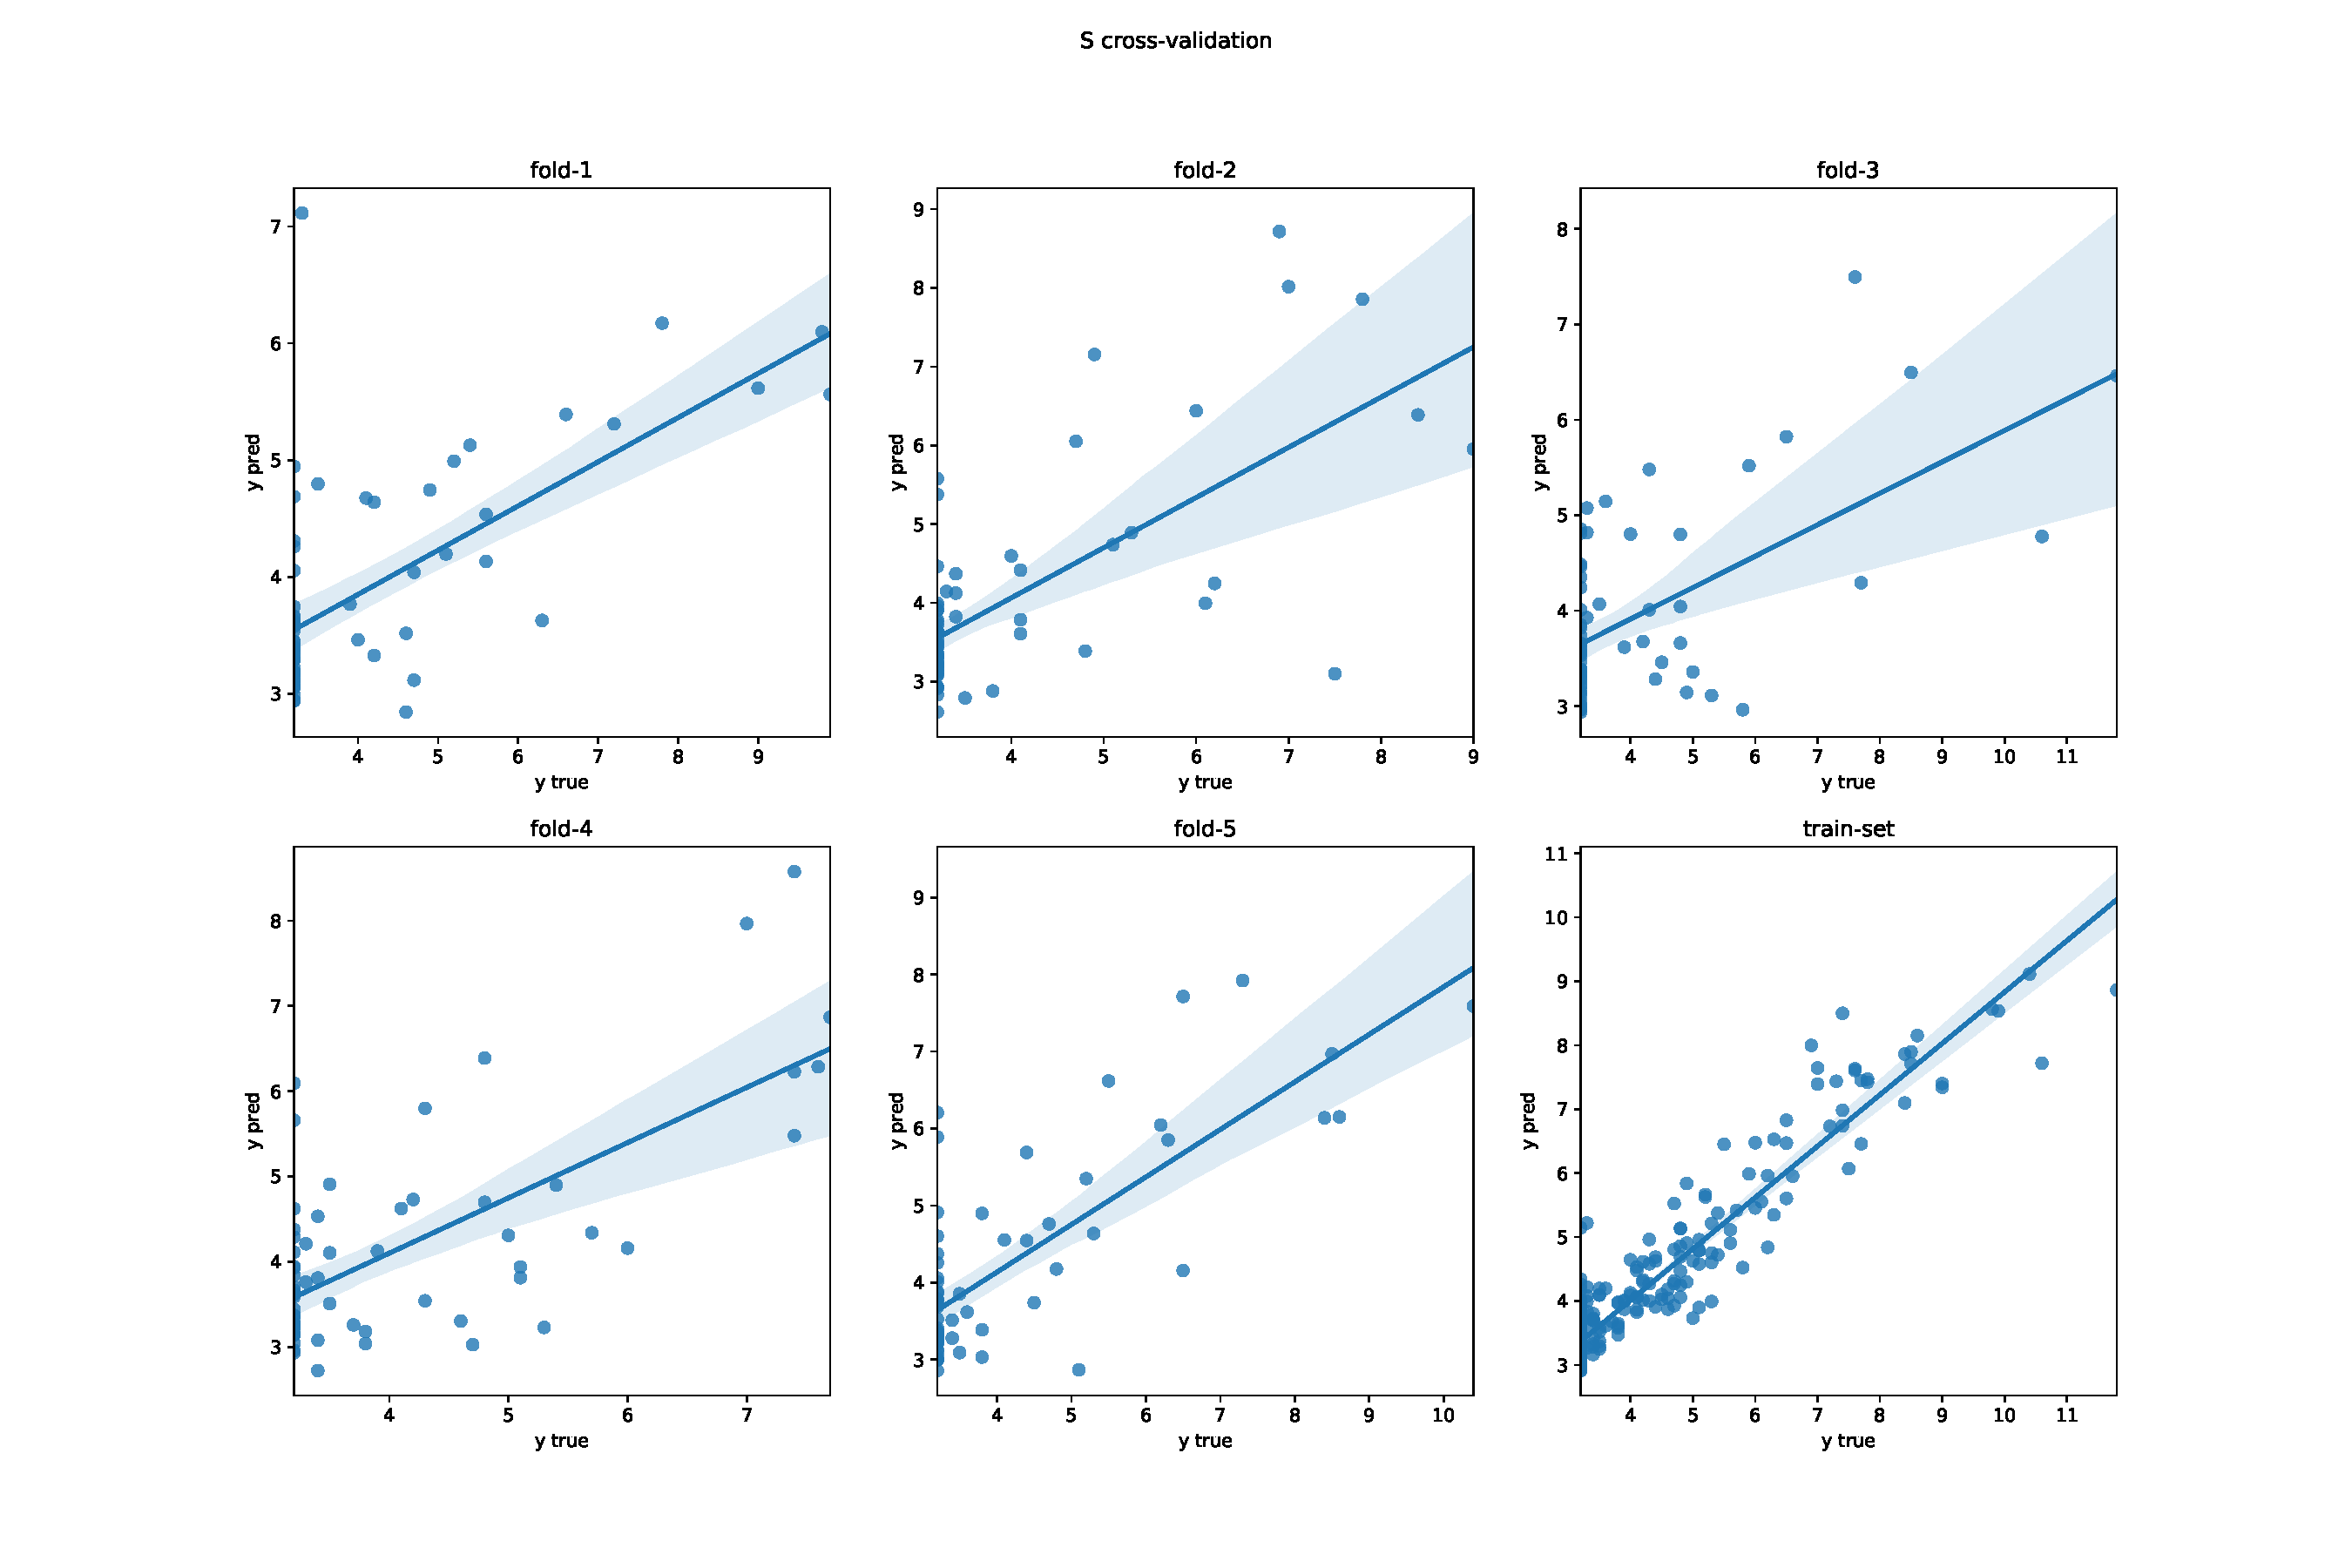
\includegraphics[width=.7\textwidth]{S-cross-validation}
	\caption{对S进行交叉验证}
\end{figure}

\subsection{问题四:主要变量操作方案的优化}





\FloatBarrier
\subsubsection{问题分析}

?????????????????????????????????
要求在保证产品硫含量不大于5μg/g的前提下,利用你们的模型获得325个数据样本(见附件四“325个数据样本数据.xlsx”)中,辛烷值(RON)损失降幅大于30%的样本对应的主要变量优化后的操作条件(优化过程中原料、待生吸附剂、再生吸附剂的性质保持不变,以它们在样本中的数据为准)。

\FloatBarrier
\subsubsection{贝叶斯优化与TPE算法简介}

\FloatBarrier
\subsubsection{对产品硫含量进行优化}

对于辛烷值进行特征筛选,选出的主要操作变量是:'稳定塔下部温度', '精制汽油出装置温度', '精制汽油出装置硫含量', '加热炉主火嘴瓦斯入口压力', 'E-101D壳程出口管温度', 'D-204液位', 'D-102温度', 'R-101下部床层压降', 'P-101B入口过滤器差压', 'F-101出口支管\#4温度', 'D101原料缓冲罐压力';对于硫进行建模,选出的主要操作变量是:'精制汽油出装置硫含量','混氢点氢气流量','还原器温度','D203出口燃料气流量','D-123压力','烟气出对流室温度','冷氮气过滤器ME-114差压','R-102底喷头压差', 两组操作变量的交集是'精制汽油出装置硫含量'。

原工业数据的产品硫含量的分布图如下,其中大于5$\mu g/g$的样本有59个,占 $18.15\%$。

\begin{figure}[htb]
	\centering
	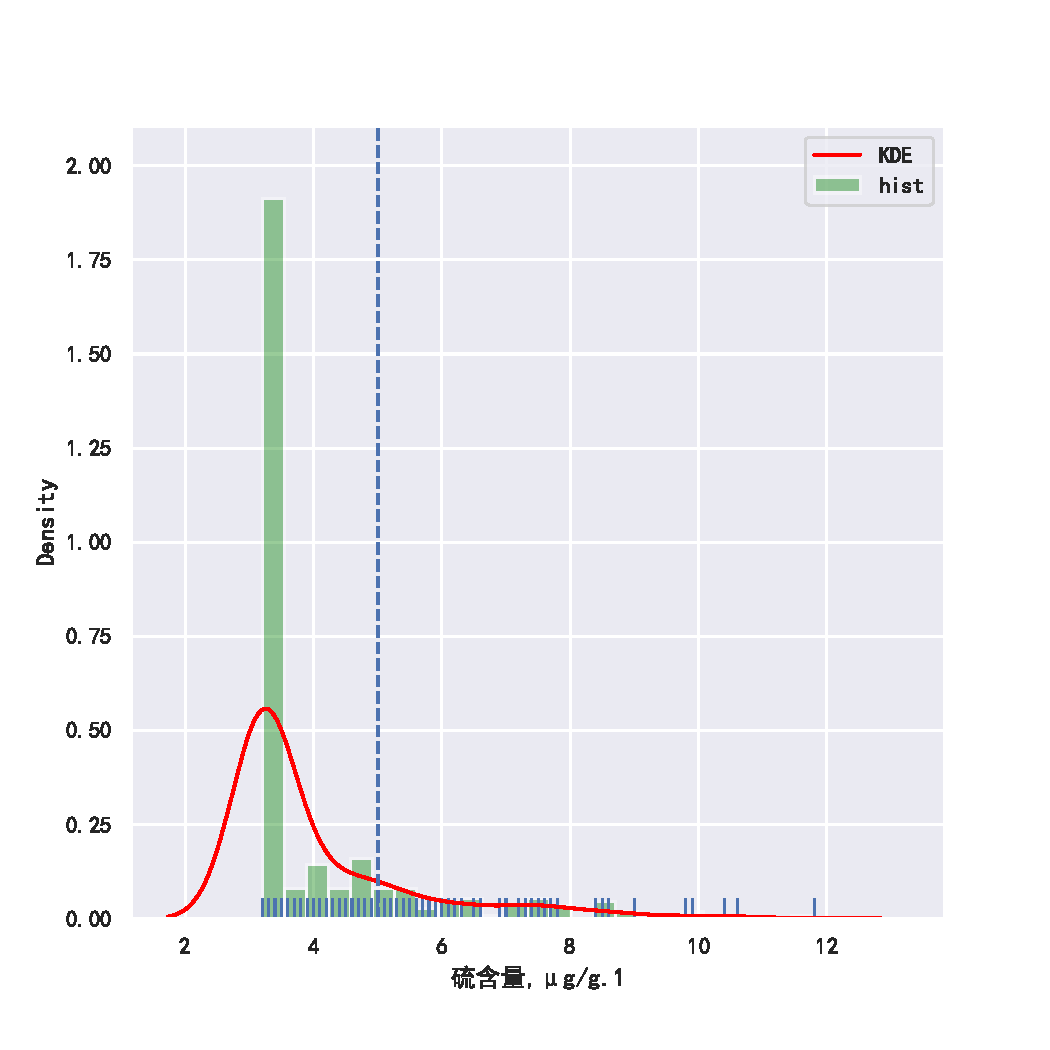
\includegraphics[width=.7\textwidth]{S-dist}
	\caption{原工业数据硫含量的分布图}
\end{figure}

我们用之前得到的硫预测模型作为评价函数,以与硫含量相关的8个主要变量作为待优化变量,并根据操作变量的取值范围得到一个参数空间,用贝叶斯优化库HyperOpt对工业数据的325个样本逐一进行优化。



\begin{figure}[htb]
	\centering
	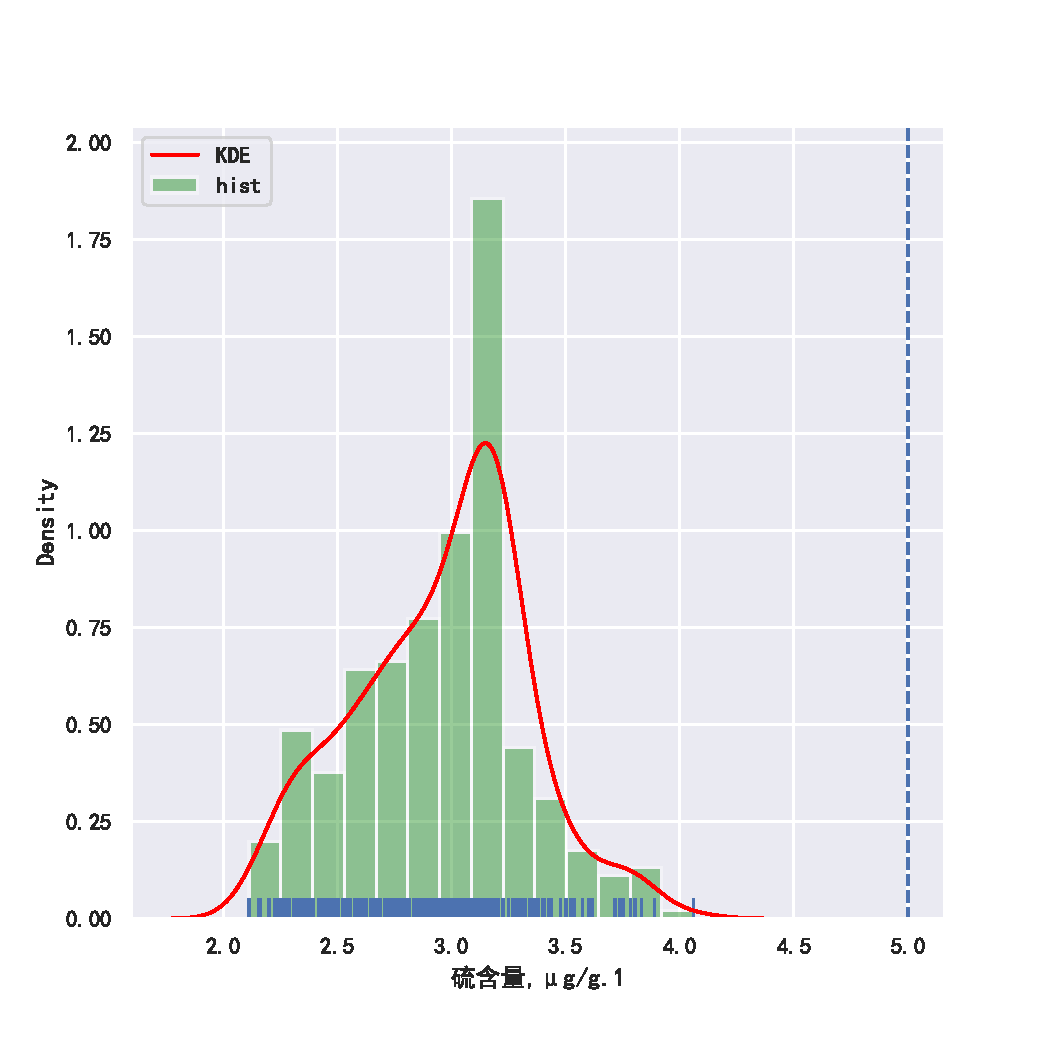
\includegraphics[width=.7\textwidth]{S-dist(after-opt)}
	\caption{单独对与硫相关的8个操作变量优化后硫含量的分布图}
\end{figure}




\FloatBarrier
\subsubsection{对辛烷损失进行优化}

\begin{figure}[htb]
	\centering
	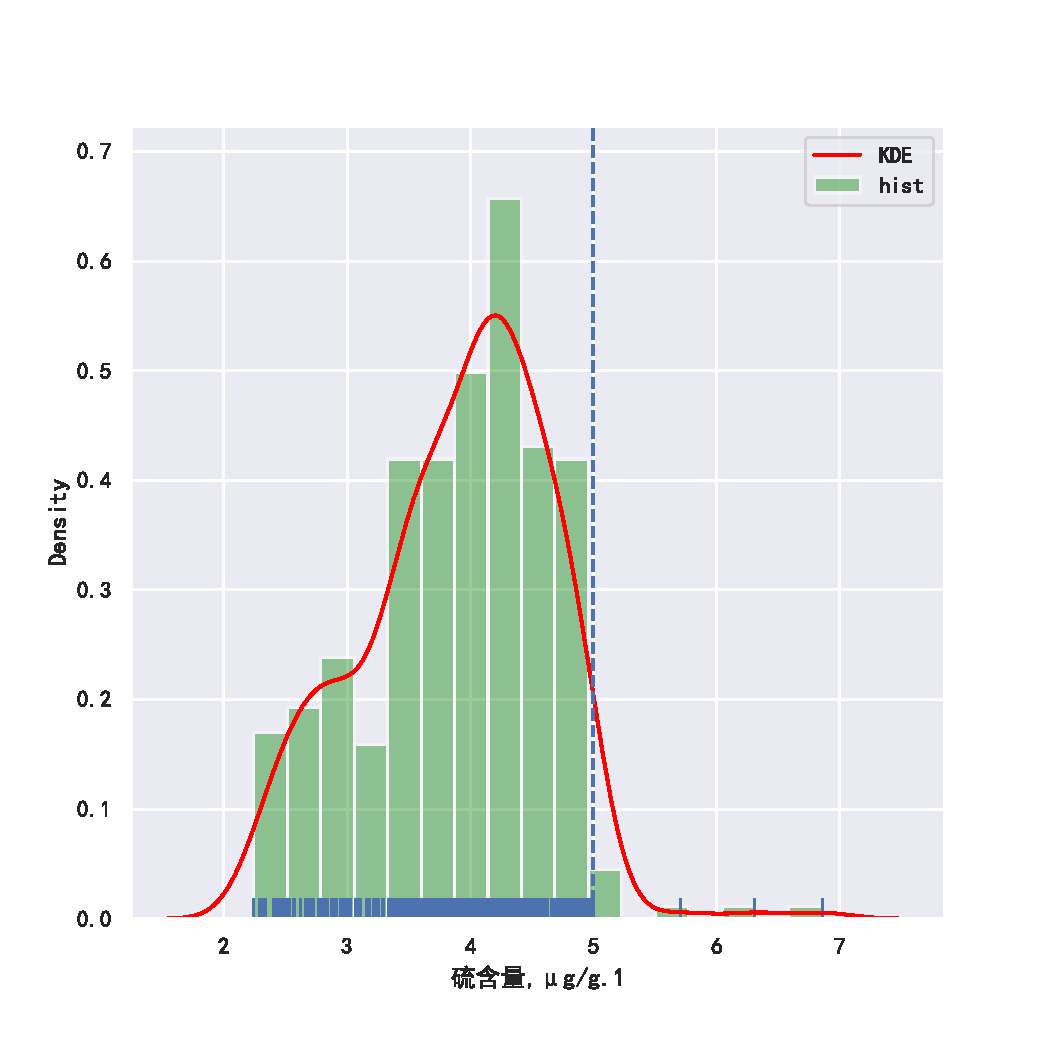
\includegraphics[width=.7\textwidth]{S-dist(after-RON-opt)}
	\caption{对RON-loss优化后硫含量的分布图}
\end{figure}

\begin{figure}[htb]
	\centering
	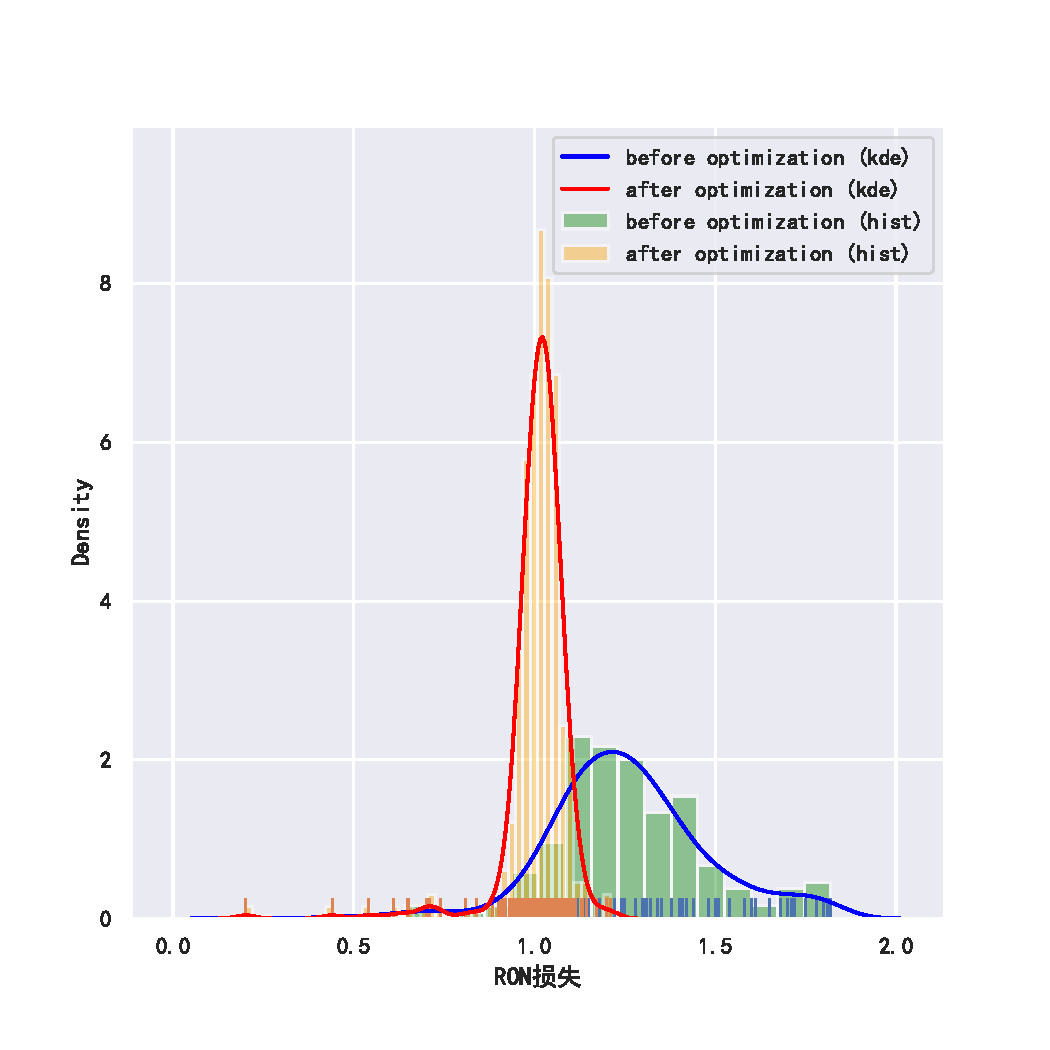
\includegraphics[width=.7\textwidth]{RON-dist}
	\caption{优化前后的RON损失分布图}
\end{figure}




\begin{figure}[htb]
	\centering
	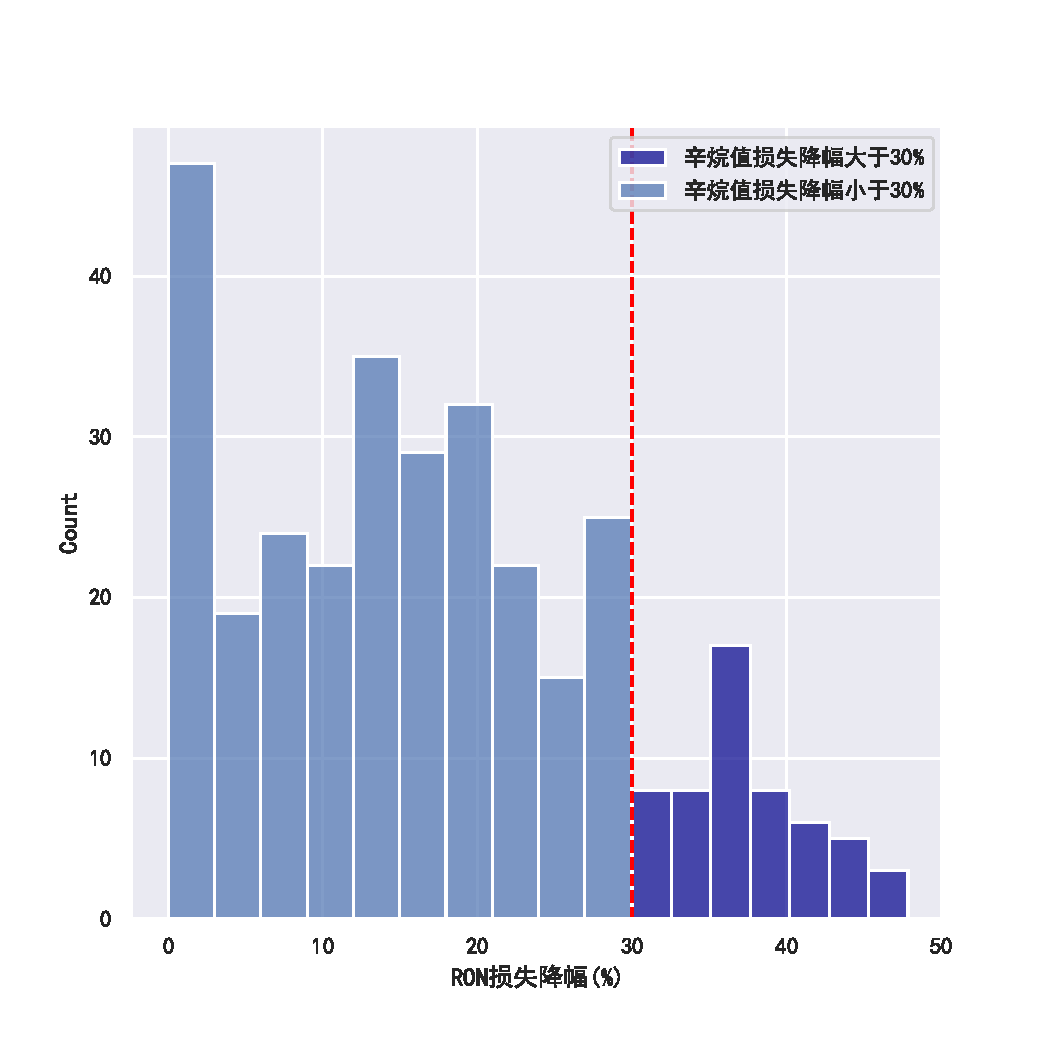
\includegraphics[width=.7\textwidth]{RON-loss-decrease}
	\caption{RON损失降幅直方图}
\end{figure}

\begin{table}[htb]
	\caption{3个优化后不符合约束条件的异常样本}\label{tab:001} \centering
	\begin{tabular}{ccccc}
		\toprule[1.5pt]
	 time &  原硫含量($\mu g/g$) &  优化后硫含($\mu g/g$) &  原RON损失 &  优化后RON损失 \\
		\midrule[1pt]
2017/11/10 8:00:00 &              4.2 &               6.30 &    1.10 &      0.99 \\
2017/11/6 8:00:00 &              6.2 &               5.70 &    1.10 &      0.91 \\
2017/9/18 8:00:00 &              3.8 &               6.86 &    1.21 &      0.89 \\  
		\bottomrule[1.5pt]
	\end{tabular}
\end{table}

\begin{figure}[htb]
	\centering
	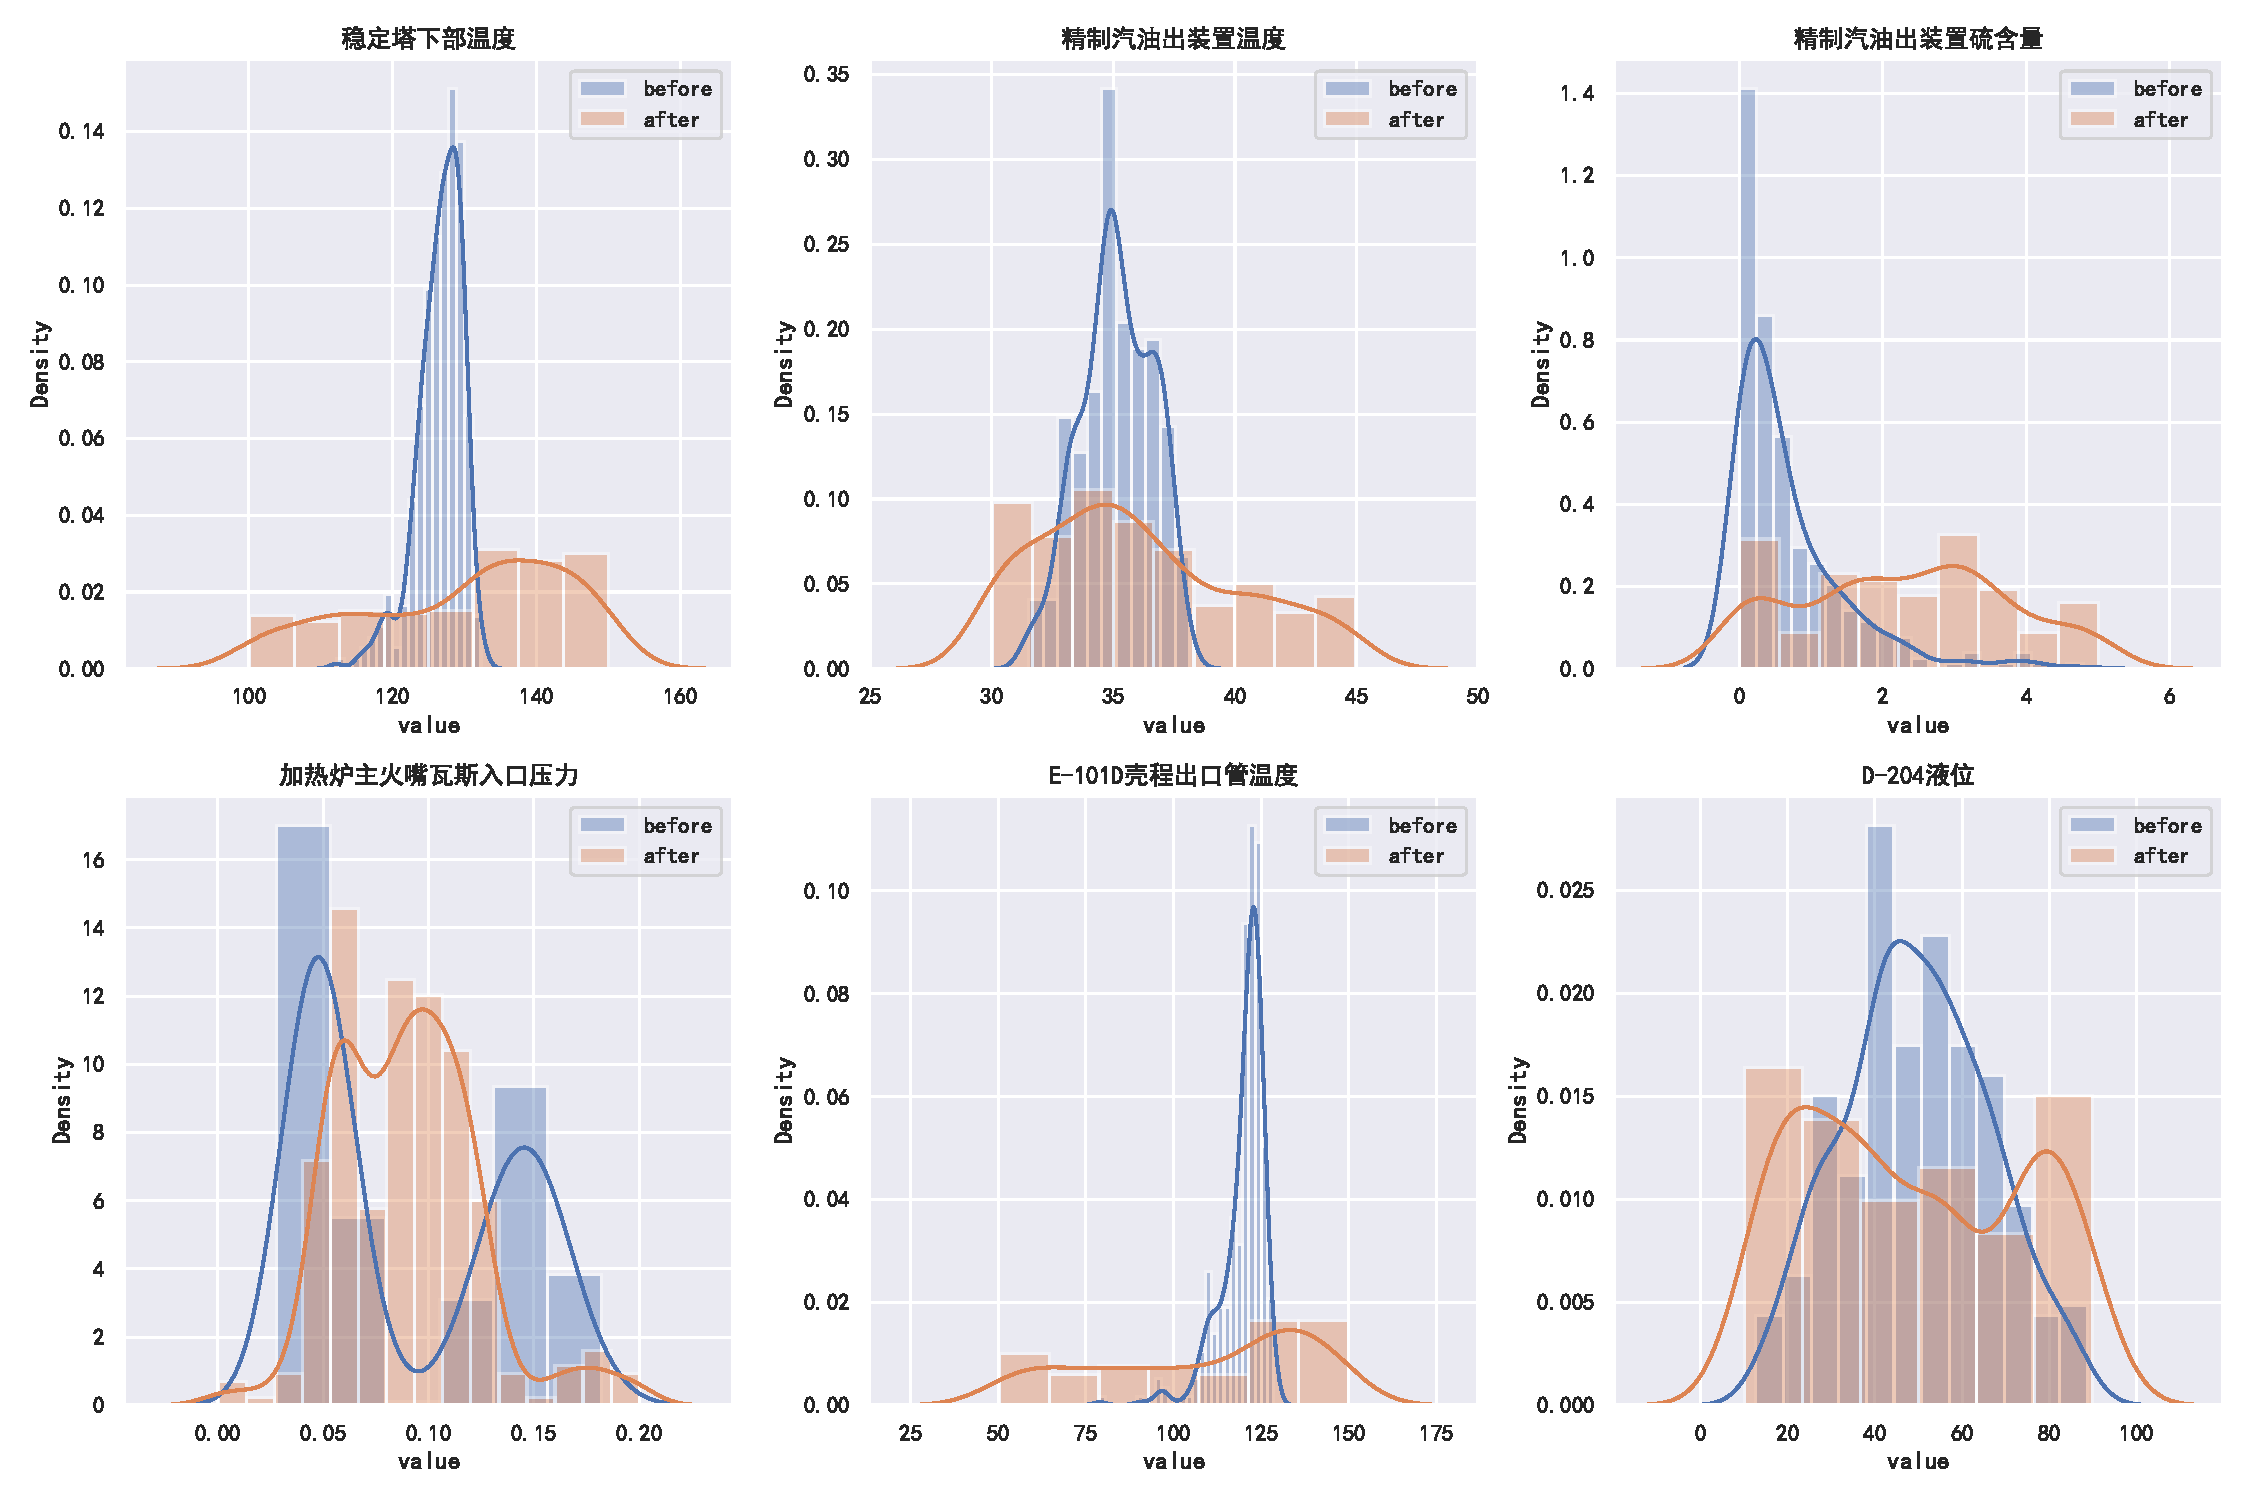
\includegraphics[width=.7\textwidth]{main-op-opt-0}
	\caption{优化前后6个操作变量的分布}
\end{figure}

\begin{figure}[htb]
	\centering
	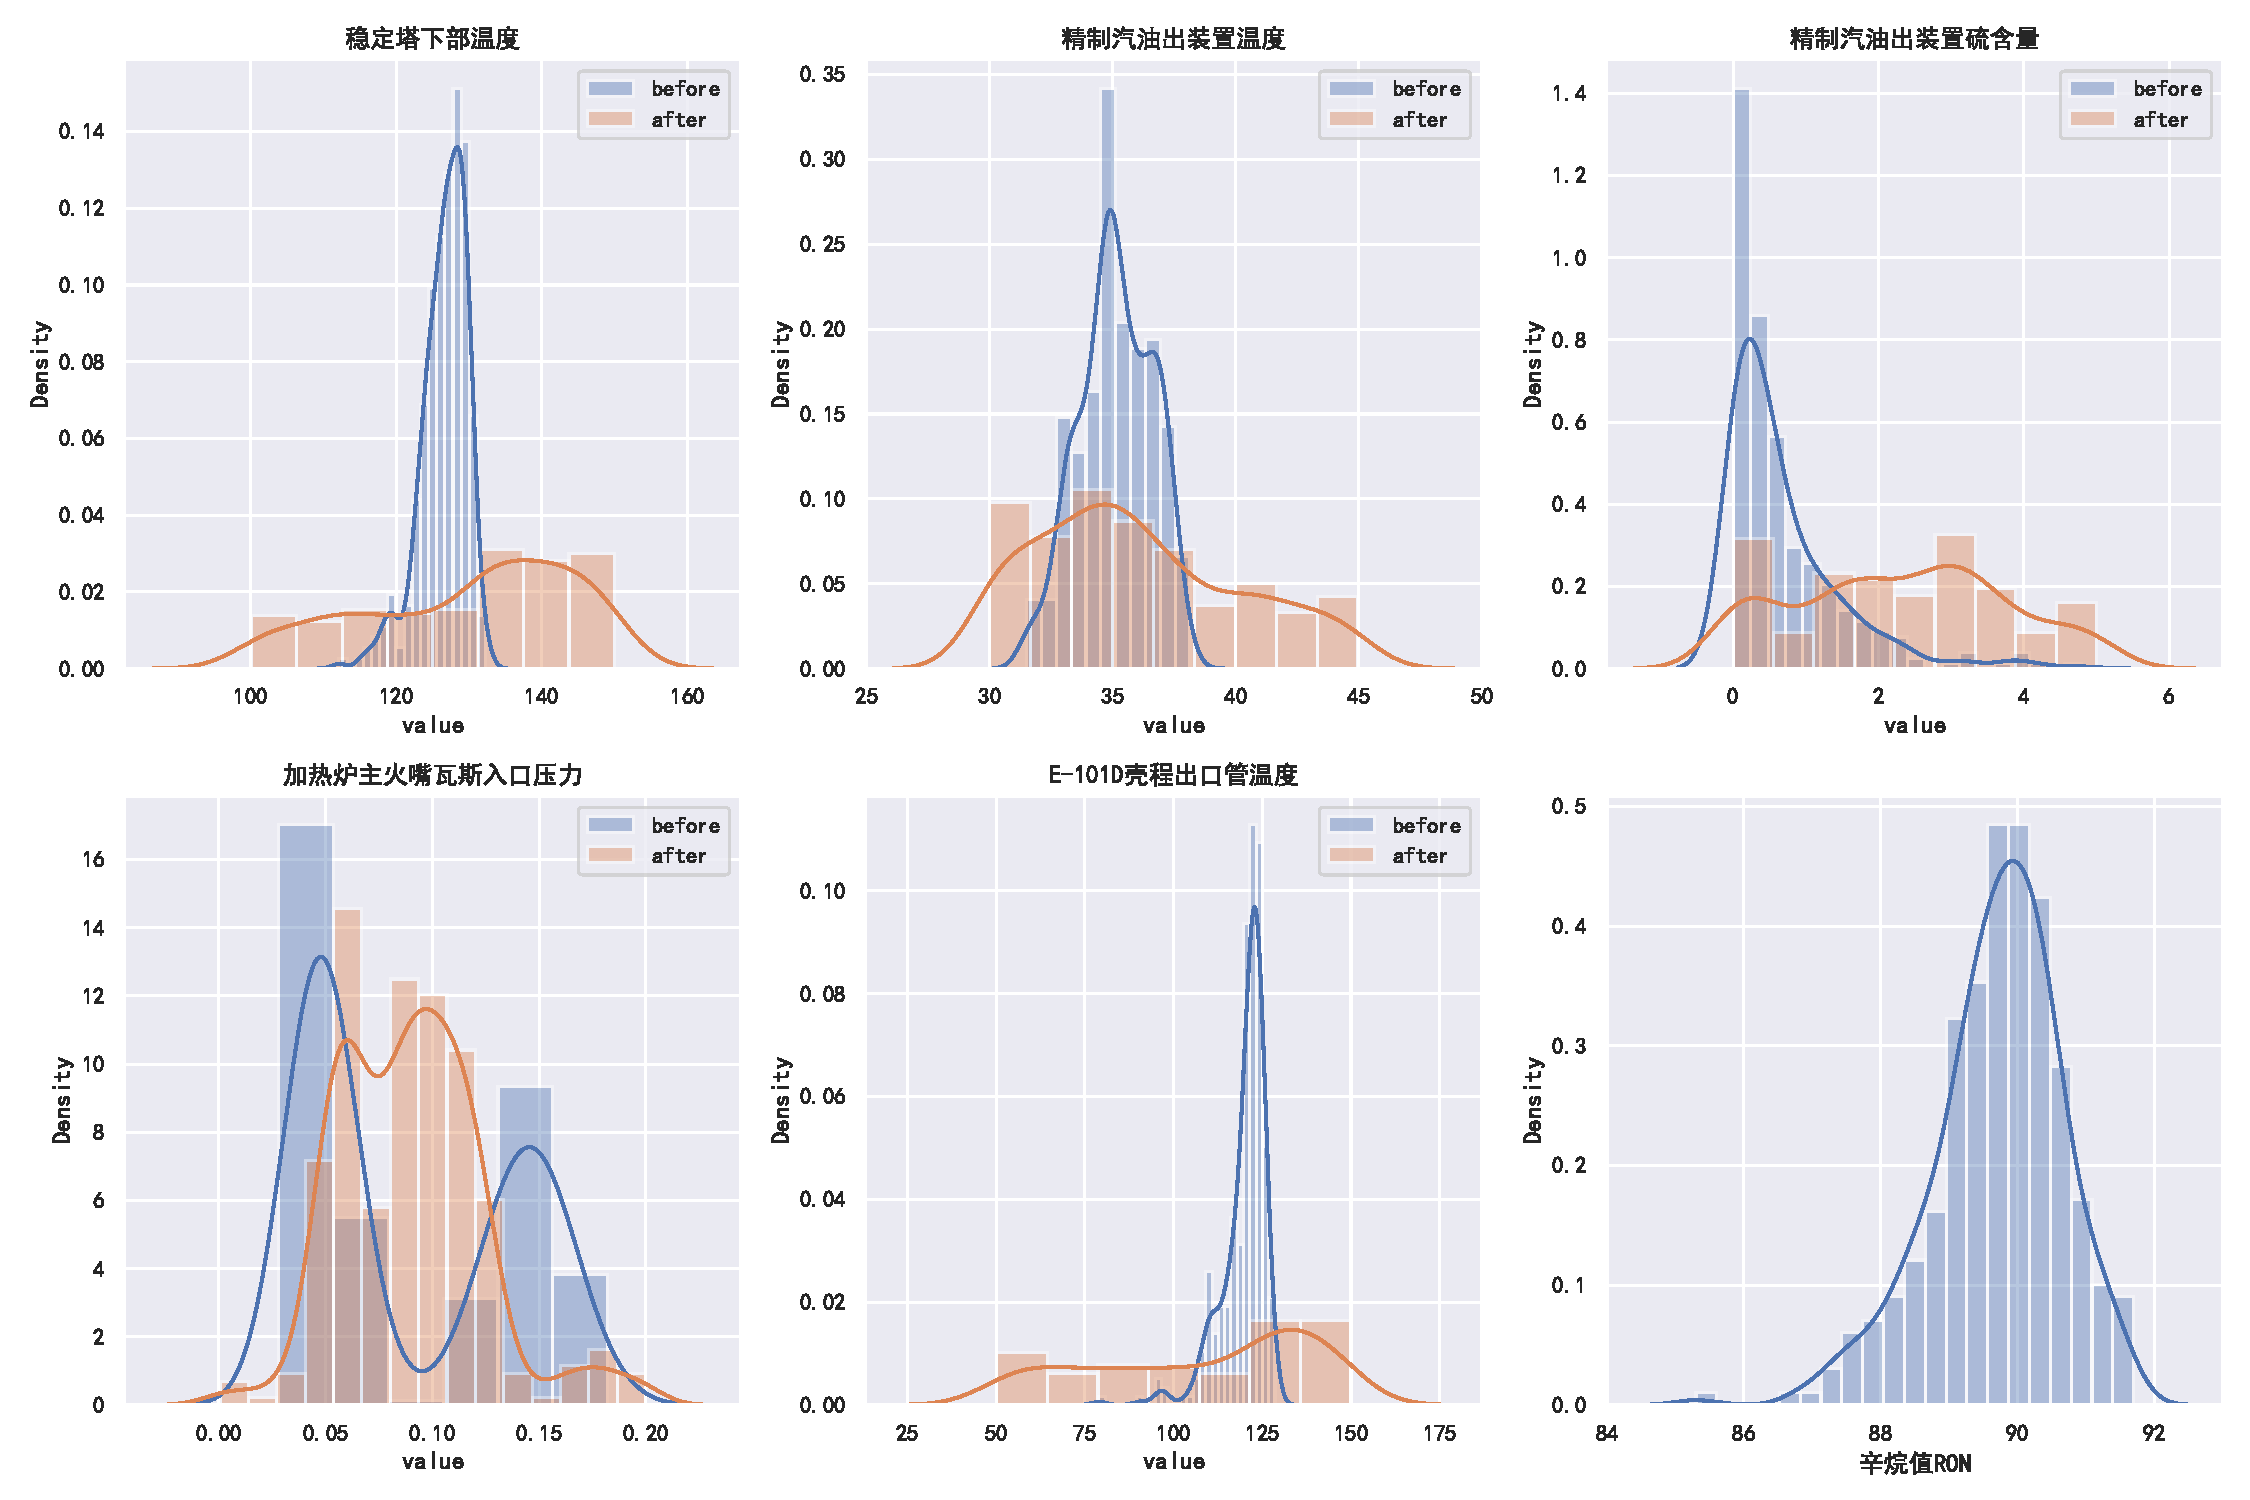
\includegraphics[width=.7\textwidth]{main-op-opt-1}
	\caption{RON与优化前后的5个操作变量的分布}
\end{figure}

\subsection{问题五:模型的可视化展示}

\FloatBarrier
\subsubsection{问题分析}

?????????????????????????????????
工业装置为了平稳生产,优化后的主要操作变量(即:问题2中的主要变量)往往只能逐步调整到位,请你们对133号样本(原料性质、待生吸附剂和再生吸附剂的性质数据保持不变,以样本中的数据为准),以图形展示其主要操作变量优化调整过程中对应的汽油辛烷值和硫含量的变化轨迹。(各主要操作变量每次允许调整幅度值Δ见附件四“354个操作变量信息.xlsx”)。



%第五章节
%下面这块看看怎么改
\FloatBarrier
\section{模型评价}


\FloatBarrier
\subsection{模型的优点}
巴拉巴拉一堆话巴拉巴拉一堆话巴拉巴拉一堆话巴拉巴拉一堆话巴拉巴拉一堆话巴拉巴拉一堆话巴拉巴拉一堆话巴拉巴拉一堆话巴拉巴拉一堆话巴拉巴拉一堆话巴拉巴拉一堆话巴拉巴拉一堆话巴拉巴拉一堆话巴拉巴拉一堆话巴拉巴拉一堆话巴拉巴拉一堆话巴拉巴拉一堆话巴拉巴拉一堆话巴拉巴拉一堆话


\FloatBarrier
\subsection{模型的缺点}
巴拉巴拉一堆话巴拉巴拉一堆话巴拉巴拉一堆话巴拉巴拉一堆话巴拉巴拉一堆话巴拉巴拉一堆话巴拉巴拉一堆话巴拉巴拉一堆话巴拉巴拉一堆话巴拉巴拉一堆话巴拉巴拉一堆话巴拉巴拉一堆话巴拉巴拉一堆话巴拉巴拉一堆话巴拉巴拉一堆话巴拉巴拉一堆话巴拉巴拉一堆话巴拉巴拉一堆话巴拉巴拉一堆话






% \section{加图的方法,记得删除}
% \begin{figure}[htb]
% \centering
% 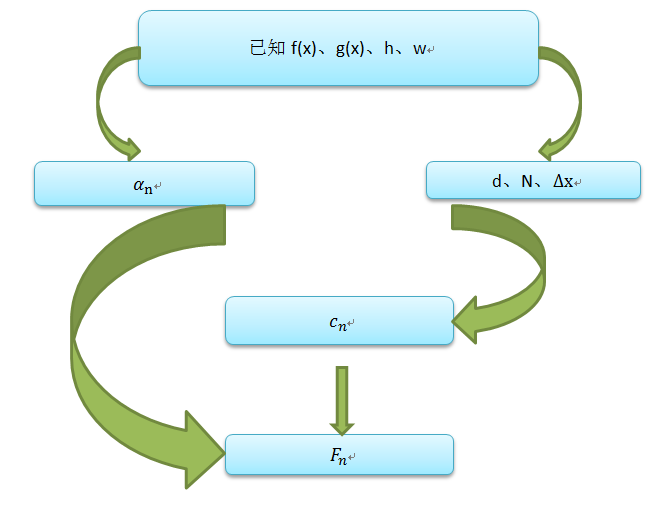
\includegraphics[width=.7\textwidth]{f1.png}
% \caption{问题三流程图}
% \end{figure}



%下面两种参考文献的格式二选一

%参考文献重新分页
\newpage

% 参考文献   手工录入
% \begin{thebibliography}{9}%宽度9
% \bibitem{bib:one} ....
% \bibitem{bib:two} ....
% \end{thebibliography}


\begin{thebibliography}{99}  
\bibitem{ref1}Zheng L, Wang S, Tian L, et al., Query-adaptive late fusion for image search and person re-identification, Proceedings of the IEEE Conference on Computer Vision and Pattern Recognition, 2015: 1741-1750.  
\bibitem{ref2}Arandjelović R, Zisserman A, Three things everyone should know to improve object retrieval, Computer Vision and Pattern Recognition (CVPR), 2012 IEEE Conference on, IEEE, 2012: 2911-2918.  
\bibitem{ref3}Lowe D G. Distinctive image features from scale-invariant keypoints, International journal of computer vision, 2004, 60(2): 91-110.  
\bibitem{ref4}Philbin J, Chum O, Isard M, et al. Lost in quantization: Improving particular object retrieval in large scale image databases, Computer Vision and Pattern Recognition, 2008. CVPR 2008, IEEE Conference on, IEEE, 2008: 1-8.  
\end{thebibliography}


% %采用bibtex方案
% \cite{mittelbach_latex_2004,wright_latex3_2009,beeton_unicode_2008,vieth_experiences_2009}

% \bibliographystyle{gmcm}
% \bibliography{example}


%参考文献 2019年大学生数学建模比赛的模板中提取的
\begin{thebibliography}{9}%宽度9
    \bibitem{1}{liuhaiyang2013latex}
    刘海洋.
    \newblock \LaTeX {}入门\allowbreak[J].
    \newblock 电子工业出版社, 北京, 2013.
    \bibitem{2}{mathematical-modeling}
    全国大学生数学建模竞赛论文格式规范 (2020 年 8 月 25 日修改).
    \bibitem{3} \url{https://www.latexstudio.net}
\end{thebibliography}






\newpage
%附录
\appendix
%\setcounter{page}{1} %如果需要可以自行重置页码。
\section{我的 Python 源程序}
\begin{lstlisting}[language=Python]%设置不同语言即可。
kk=2;[mdd,ndd]=size(dd);
while ~isempty(V)
[tmpd,j]=min(W(i,V));tmpj=V(j);
for k=2:ndd
[tmp1,jj]=min(dd(1,k)+W(dd(2,k),V));
tmp2=V(jj);tt(k-1,:)=[tmp1,tmp2,jj];
end
tmp=[tmpd,tmpj,j;tt];[tmp3,tmp4]=min(tmp(:,1));
if tmp3==tmpd, ss(1:2,kk)=[i;tmp(tmp4,2)];
else,tmp5=find(ss(:,tmp4)~=0);tmp6=length(tmp5);
if dd(2,tmp4)==ss(tmp6,tmp4)
ss(1:tmp6+1,kk)=[ss(tmp5,tmp4);tmp(tmp4,2)];
else, ss(1:3,kk)=[i;dd(2,tmp4);tmp(tmp4,2)];
end;end
dd=[dd,[tmp3;tmp(tmp4,2)]];V(tmp(tmp4,3))=[];
[mdd,ndd]=size(dd);kk=kk+1;
end; S=ss; D=dd(1,:);


 \end{lstlisting}


\end{document} 